\documentclass[main.tex]{subfiles}

\usepackage{graphicx}
\usepackage{slashed}
\usepackage{color}
%\usepackage{amsmath}
%\usepackage{amssymb}

\definecolor{mypink}{RGB}{219, 48, 122}
\definecolor{mygreen}{rgb}{0,0.7,0}
\def\SB#1{\textcolor{mygreen}{{\bf\tt [SB: #1]}}}
\def\TP#1{\textcolor{yellow}{{\bf\tt [TP: #1]}}}
\def\BH#1{\textcolor{red}{{\bf\tt [BH: #1]}}}
\def\EC#1{\textcolor{mypink}{{\bf\tt [EC: #1]}}}
\def\SZ#1{\textcolor{blue}{{\bf\tt [SZ: #1]}}}
\def\JK#1{\textcolor{cyan}{{\bf\tt [JK: #1]}}}
\def\txB#1{\textcolor{blue}{#1}}

%%% spinor products %%%

\def\finite{\mathrm{finite}}
\def\renorm{\mathrm{ren,CDR}}
\def\irpole{\mathrm{pole,CDR}}
 
\def\fin{\mathrm{fin}}
\def\zz{\boldsymbol{Z}}
\def\mi{\mathrm{MI}}
\def\cF{\mathcal{F}}
\def\cP{\mathcal{P}}
\def\cC{\mathcal{C}}
\def\cA{\mathcal{A}}
\def\cN{\mathcal{N}}
\def\cO{\mathcal{O}}
\def\cD{\mathcal{D}}
\def\cQ{\mathcal{Q}}
\def\cJ{\mathcal{J}}
\def\cI{\mathcal{I}}
\def\cT{\mathcal{T}}
\def\nn{\nonumber \\ }

\def\wpol{\varepsilon_W}
\def\lrbrace#1{\lbrace#1\rbrace}
\def\la{\langle}
\def\ra{\rangle}
\def\spA#1#2{\la#1#2\ra}
\def\spB#1#2{[#1#2]}
\def\spAB#1#2#3{\la#1|#2|#3]}
\def\spBA#1#2#3{[#1|#2|#3\ra}
\def\spAA#1#2#3{\la#1|#2|#3\ra}
\def\spBB#1#2#3{[#1|#2|#3]}
\def\spab#1#2{\la#1|#2]}
\def\spaa#1#2#3#4{\la#1|#2|#3|#4\ra}
\def\spbb#1#2#3#4{[#1|#2|#3|#4]}
\def\wh#1{\widehat#1}
%\DeclareMathOperator{\tr}{\rm tr}
%\def\trm{\tr_-}
%\def\trp{\tr_+}
\def\MP#1#2{(#1\cdot#2)}
%\def\trfive{\tr_5}
\def\spAXB#1#2#3#4#5{\la#1|#2|#3|#4|#5]}

\def\bra#1{\langle #1|}
\def\ket#1{|#1 \rangle}
\def\sqbra#1{[#1|}
\def\sqket#1{|#1]}
\def\braket#1{\langle #1 \rangle}

\def\eps{\epsilon}
\def\fl#1{#1^\flat}
\def\tl#1{\tilde{#1}}
\def\wh{\widehat}
\def\tC{\tilde{C}}
\def\qb{{\bar{q}}}
\def\sb{\bar{s}}
\def\Sb{\bar{S}}
\def\lb{\bar{\ell}}
\def\tb{{\bar{t}}}
\def\ttgg{\bar{t}tgg}
\def\mren{\mathrm{mren}}
\def\ren{\mathrm{ren}}
\def\mct{\mathrm{mct}}
\def\ceps{C_\eps}
\def\as{\alpha_s}
\def\dk#1{\frac{d^d k_{#1}}{i\pi^{d/2}e^{-\eps \gamma_E}}}
\def\bbh{b\bar{b}H}
\def\bbggh{\bar{b}bggH}
\def\bbqqh{\bar{b}b\bar{q}qH}

\def\e{\epsilon}
\def\tT{\tilde{T}}
\def\coll#1#2{\overset{#1||#2}{\to}}
\def\inf{{\rm Inf}}
%\def\gg#1{\gamma_{#1}}
\def\XX{\chi}

\def\cv#1#2{\AB{#1}{\gamma^\mu}{#2}}
\def\cvS#1#2#3{\AB{#1}{#2}{#3}}

\def\MHVb{$\overline{\rm MHV}$}
\def\boxX{$\xcancel{\rm\bf box}$}

\def\fl#1{{#1^{\flat}}}
\def\flm#1{{#1^{\flat,\mu}}}
\def\kf#1{{\fl{K_{#1}}}}
\def\kfm#1{{\flm{K_{#1}}}}

\def\ulim#1{\underset{#1}{\lim}}

\def\fbox#1{F^{(#1)}_{\mathrm{box}}}
\def\lh{\hat{L}}
\def\li#1{\mathrm{Li}_{#1}}

\def\finr{{\mathcal{F}}}
\def\pole{{\mathcal{P}}}
\def\cusp{{\mathrm{cusp}}}
\def\sumhel{\sum_{\mathrm{helicity}}}

%%%% typesetting equations %%%%
\def\s#1{s_{#1}}
\def\d#1#2{#1\cdot #2}
\def\p#1{#1}
\def\pp#1{p_{#1}}
\def\f#1{#1^\flat}
\def\n#1{\eta_{#1}}

\def\Adcc{B_n^{(1)}}

\def\usepic#1#2{\parbox{#1}{\includegraphics[width=#1]{#2}}}
\def\usepix#1#2#3#4#5#6{\parbox{#1}{\includegraphics[width=#1,trim= #3 #4 #5 #6,clip=true]{#2}}}

\def\hpl11{{\mathrm{HPL}}_{1,1}}

\tikzset{cross/.style={cross out, draw, 
         minimum size=2*(#1-\pgflinewidth), 
         inner sep=0pt, outer sep=0pt}}
\newcolumntype{C}[1]{>{\hsize=#1\hsize\centering\arraybackslash}X}

\begin{document}
\chapter{Two-loop helicity amplitudes for $\ppbbh$ production} \label{sec:Hbb}
In this chapter, we present the computation of the two-loop QCD helicity amplitudes for the production of a Higgs boson in association with a bottom quark pair at a hadron collider. We take the approximation of leading colour and work in the five flavour scheme, where the bottom quarks are massless while the Yukawa coupling is non-zero. We extract analytic expressions from multiple numerical evaluations over finite fields and present the results in terms of an independent set of special functions that can be reliably evaluated over the full phase space.

The chapter is organised as follows. After providing the necessary background and context in which this work is situated, in Section~\ref{Hbbsec:amp} we describe the structure of the $b\bar{b}H$ amplitudes at leading colour, followed by a brief outline of the methodology used in deriving the analytic expression of the amplitudes in Section~\ref{Hbbsec:reduction}. A description of the basis of special functions is presented in Section~\ref{Hbbsec:Hbasis} and a number of validations that we performed on the results derived in this work are discussed in Section~\ref{Hbbsec:validation}. We present benchmark numerical evaluations together with evaluations on a physical phase space slice in Section~\ref{Hbbsec:results}. Finally, we draw our conclusions in Section~\ref{Hbbsec:conclusions}. 
\section{Introduction \label{Hbbsec:intro}}
%Precise theoretical predictions are an essential ingredient in the search for subtle deviations from
%the Standard Model (SM) at current and future collider experiments. The enormous amount of data
%gathered at the Large Hadron Collider (LHC) is already challenging the theoretical precision for
%many processes and the pressure will increase as data continues to pour in. It has been clear for
%some time~\cite{Badger:2016bpw,Bendavid:2018nar,Amoroso:2020lgh} that, for a large class of two- and three-particle final states, at least the Next-to-Next-to-Leading Order corrections in Quantum Chromodynamics (NNLO QCD) will be required for fully differential cross sections. The high multiplicity final states, particularly those with many kinematic scales, pose the biggest technical challenge owing to the enormous analytic and algebraic complexity. Nevertheless, thanks to a huge effort across the theoretical community, new tools and methods have been developed that have produced the first NNLO QCD predictions for $2\to3$ processes~\cite{Chawdhry:2019bji,Kallweit:2020gcp,Chawdhry:2021hkp}, most notably for 3-jet production~\cite{Czakon:2021mjy}. This remarkable progress has been driven both by the advancements in the scattering amplitude computation and by efficient subtraction schemes. By now, all the two-loop MIs --~which are one of the important ingredients in the amplitude computation~-- are available for the fully massless five-particle processes~\cite{Papadopoulos:2015jft, Gehrmann:2018yef, Abreu:2018rcw, Chicherin:2018mue, Chicherin:2018old, Chicherin:2020oor}, allowing for several two-loop QCD amplitudes to be derived
%analytically~\cite{Gehrmann:2015bfy, Badger:2018enw, Abreu:2018zmy,Abreu:2019odu, Badger:2019djh, Abreu:2020cwb, Chawdhry:2020for, Agarwal:2021grm, Abreu:2021fuk, Chawdhry:2021mkw, Agarwal:2021vdh, Badger:2021imn}, improving on previous results that were obtained numerically~\cite{Badger:2017jhb, Abreu:2017hqn, Badger:2018gip, Abreu:2018jgq}. These new results have been achieved thanks to technological breakthroughs in the method of differential
%equations~\cite{Kotikov:1990kg, Bern:1993kr, Remiddi:1997ny, Gehrmann:1999as, Henn:2013pwa}, integral reduction algorithms~\cite{Gluza:2010ws, Schabinger:2011dz, Ita:2015tya, Larsen:2015ped, Boehm:2017wjc} and the use of finite-field arithmetic to tame the algebraic complexity of multi-leg and multi-scale problems~\cite{vonManteuffel:2014ixa, Peraro:2016wsq, Klappert:2019emp, Peraro:2019svx, Klappert:2020aqs, Klappert:2020nbg}.
%
%A different class of $2\to 3$ processes that is of great interest involves an external massive leg.
%The two-loop planar helicity amplitudes for $W+4$-parton scattering (contributing to the prediction
%for $W+2$-jet production at NNLO QCD) have been previously studied numerically~\cite{Hartanto:2019uvl}. 
%All two-loop integrals needed for this type of process are available for the planar
%contributions~\cite{Papadopoulos:2015jft,Abreu:2020jxa,Canko:2020ylt,Syrrakos:2020kba}, and the
%first analytic result was derived for $Wb\bar{b}$ production in the leading colour, massless
%$b$-quark and on-shell $W$-boson approximations~\cite{Badger:2021nhg}. 
%Very recently, complete analytic results for one of the non-planar integral topologies have also become available~\cite{Papadopoulos:2019iam,abreu2021twoloop}.

Form the perspective of phenomenology, $\ppbbh$ production at the LHC has been a subject of great interest due to its
potential in directly measuring the bottom-quark Yukawa coupling. In the SM, the
coupling strengths of the Higgs boson to the fermions and vector bosons are proportional to their
mass, causing the rate of the $b\bar{b}H$ production to be suppressed with respect to, for example,
Higgs production in gluon fusion ($gg\to H$) or vector boson fusion ($pp\to Hjj$), associated
production with a vector boson ($pp\to VH$), and associated production with a top-quark pair ($pp\to
t\bar{t}H$). In addition, the presence of $b$-tagging further suppresses the $b\bar{b}H$ production
rate.  In some new physics scenarios, such as the Two Higgs Doublet Models (2HDM's) and the Minimal
Supersymmetric Standard Model (MSSM), the bottom-quark Yukawa coupling can be dramatically enhanced,
resulting in a considerable increase of the $b\bar{b}H$ production
rate~\cite{Balazs:1998nt,Dawson:2005vi}.  Thus, the study of the $b\bar{b}H$ production will allow
to constrain supersymmetric models and other extensions of the SM that modify the bottom-quark
Yukawa coupling. Recent studies on the interplay between $b\bar{b}H$ signal and backgrounds can be
found in Refs.~\cite{Pagani:2020rsg,Grojean:2020ech,Konar:2021nkk}.

The theoretical approach to obtaining predictions for the $pp\to b\bar{b}H$ process has been subject
of much discussion in the community. This is due to the fact that, in the presence of bottom quarks,
a theoretical prediction can be computed in either the four-flavour scheme (4FS) or the five-flavour
scheme (5FS). In the 4FS computation, bottom quarks are treated as massive and they do not
contribute to the PDFs, hence only appearing in the final state.
Large logarithms of the form $\log(m_b/Q)$ with $Q \propto m_H$ arise when the integration over the
bottom-quark phase space is performed, and such contributions may spoil the convergence of the
perturbative series. These large logarithms can be resummed to all orders by introducing the
bottom quark PDFs.  The 5FS approach stems from this prescription, where
the bottom quarks are included in the PDFs, allowed to appear in the
initial state, and treated as massless.  We refer the reader to Ref.~\cite{Maltoni:2012pa} for further
discussion on the 5FS and 4FS approaches. 
In 5FS, the inclusive $b\bar{b}H$ production (where the tree level process is $b\bar{b}\to H$) has been computed up to
N3LO QCD~\cite{Dicus:1998hs,Balazs:1998sb,Maltoni:2003pn,Harlander:2010cz,Buehler:2012cu,Harlander:2012pb,H:2019nsw,Duhr:2019kwi,Mondini:2021nck}, 
while for the case where a single bottom quark is observed NLO QCD~\cite{Campbell:2002zm}, weak~\cite{Dawson:2010yz} 
and SUSY QCD~\cite{Dawson:2011pe} corrections are available.
In 4FS the $b\bar{b}H$ production has been calculated up to 
NLO QCD~\cite{Dittmaier:2003ej,Dawson:2003kb,Dawson:2004sh,Wiesemann:2014ioa,Jager:2015hka,Deutschmann:2018avk},
and the supersymmetric QCD corrections~\cite{Liu:2012qu,Dittmaier:2014sva} are also known.  
There have also been efforts in matching the 5FS and 4FS calculations to obtain accurate predictions across the entire kinematic region~\cite{Harlander:2011aa,Bonvini:2015pxa,Forte:2015hba,Forte:2016sja,Duhr:2020kzd}. 
A first step towards a massive version of the five-flavour scheme (5FMS) has been devised to naturally connect the 4FS and 5FS approaches~\cite{Krauss:2017wmx,Figueroa:2018chn}.

In the following, we compute the two-loop QCD corrections to the $gg \rightarrow b\bar{b}H$,
$q\bar{q}/\bar{q}q \rightarrow b\bar{b}H$, $b\bar{b}/\bar{b}b\rightarrow b\bar{b}H$, $bb \rightarrow
bbH$ and $\bar{b}\bar{b}\rightarrow\bar{b}\bar{b}H$ reactions in the 5FS. These two-loop amplitudes
enter the computation of $pp(b\bar{b})\to H$ at N4LO, $pp\to b(\bar{b})H$ at N3LO when one $b$-jet
is tagged, and $pp\to b\bar{b}H$ at NNLO when two $b$-jets are required in the final state.  We note
that beyond NLO, for the computation with massless bottom quarks, a flavoured jet
algorithm~\cite{Banfi:2006hf} would have to be employed when identifying the $b$-jets, since the use
of conventional $k_T$ or anti-$k_T$ jet algorithms would render the fixed order computation infrared
unsafe.  We further remark that the two-loop amplitudes for $b\bar{b}H$ production derived here can also be used in the computation of Higgs decaying into a bottom quark pair in 5FS, by
crossing initial partons to the final state. Specifically, they will contribute in the N4LO $H\to
b\bar{b}$, N3LO $H\to b\bar{b}j$ and NNLO $H\to b\bar{b}jj$ computations.  In addition, by crossing
the $b\bar{b}$ pair to the initial state and the $gg/q\bar{q}$ pair to the final state we obtain the
contribution of the bottom quark initiated channel to $H+2j$ production ($b\bar{b}\to Hjj$).

We present analytic results for the finite remainders after both UV and IR poles have been subtracted. This is possible using a basis of special functions recently identified in the context
of $Wb\bar{b}$ production~\cite{Badger:2021nhg}. We obtain numerical results valid across the full phase
space by applying the generalised series expansion approach~\cite{Francesco:2019yqt,Abreu:2020jxa,Hidding:2020ytt} to the DEs satisfied by the special functions appearing in the finite remainders.

\section{Structure of the $pp\to\bbh$ Amplitudes at Leading Colour}
\label{Hbbsec:amp}
We compute the two-loop QCD corrections in the leading colour approximation for the following subprocesses:
\begin{align} \label{eq:subprocesses}
& 0 \rightarrow \bar{b}(p_1) + b(p_2) + g(p_3) + g(p_4) + H(p_5)\,, \\
& 0 \rightarrow \bar{b}(p_1) + b(p_2) + \bar{q}(p_3) + q(p_4) + H(p_5)\,, \label{eq:subprocessqq} \\
& 0 \rightarrow \bar{b}(p_1) + b(p_2) + \bar{b}(p_3) + b(p_4) + H(p_5) \,, \label{eq:subprocessbb}
\end{align}
where all momenta are taken as outgoing:
\begin{align}
\sum_{i=1}^5 p_i = 0\,.
\end{align}
We work in the 5FS, where the bottom quark is taken as massless while its Yukawa coupling to the Higgs boson is kept finite, so that:
\begin{align}
p_1^2=p_2^2=p_3^2=p_4^2=0\,, \qquad \quad p_5^2=m_H^2\,, 
\end{align}
where $m_H$ is the mass of the Higgs boson. The kinematics is described by six independent scalar products, which we choose as:
\begin{equation}
 (s_{12},s_{23},s_{34},s_{45},s_{15},p_5^2) \,, \nonumber
\end{equation}
with $s_{ij} = (p_i + p_j)^2$. It is also possible to form pseudo-scalar invariants by contracting the Levi-Civita symbol $\eps_{\mu \nu \rho \sigma}$ with any four external momenta. The five-particle kinematics is therefore fully determined by the scalar invariants above and by one pseudo-scalar invariant, which captures all the space-time parity information of the phase space. We choose:
\begin{align} \label{eq:tr5}
\text{tr}_5 = 4 i \epsilon_{\mu \nu \rho \sigma} p_1^{\mu} p_2^{\nu} p_3^{\rho} p_4^{\sigma} = [12] \spA{2}{3} [34] \spA{4}{1} - \spA{1}{2} [23] \spA{3}{4} [41] \,.
\end{align}
It is related to the scalar invariants through:
\begin{align} \label{eq:tr5squared}
\tr_5^2 =  \Delta_5 := \text{det}\left(2 p_i \cdot p_j \right)\bigl|_{i,j=1,\ldots,4} \,,
\end{align}
where the right-hand side is a degree-four polynomial in the scalar invariants.

The colour decomposition of the $L$-loop amplitudes in the leading colour approximation is given by:
\begin{align}
&\mathcal{A}^{(L)}(1_{\bar b},2_{b},3_{g},4_{g} ,5_{H}) = n^L g_s^2 y_b \bigg[ 
  (T^{a_3} T^{a_4})_{i_2}^{\;\;\bar i_1} \,  A^{(L)}(1_{\bar b},2_{b},3_{g},4_{g} ,5_{H}) + ( 3 \leftrightarrow 4 ) \bigg]\,, \nonumber\\
&\mathcal{A}^{(L)}(1_{\bar b},2_{b},3_{\bar{q}},4_{q} ,5_{H}) = n^L  g_s^2 y_b 
 \delta_{i_4}^{\;\;\bar i_1} \delta_{i_2}^{\;\;\bar i_3}  \,
  A^{(L)}(1_{\bar b},2_{b},3_{\bar{q}},4_{q} ,5_{H}) \,,  \label{eq:colourdecomposition} \\
&\mathcal{A}^{(L)}(1_{\bar b},2_{b},3_{\bar{b}},4_{b} ,5_{H}) = n^L  g_s^2 y_b \bigg[
  \delta_{i_4}^{\;\;\bar i_1} \delta_{i_2}^{\;\;\bar i_3}  \, \biggl( A^{(L)}(1_{\bar b},2_{b},3_{\bar{q}},4_{q} ,5_{H}) + A^{(L)}(3_{\bar b},4_{b},1_{\bar{q}},2_{q} ,5_{H}) \biggr) \,  \nonumber\\
& \hspace{4.5cm} -\delta_{i_2}^{\;\;\bar i_1} \delta_{i_4}^{\;\;\bar i_3}  \, \biggl( A^{(L)}(1_{\bar b},4_{b},3_{\bar{q}},2_{q} ,5_{H}) + A^{(L)}(3_{\bar b},2_{b},1_{\bar{q}},4_{q} ,5_{H}) \biggr) \bigg]\,, 
\nonumber 
\end{align}
where $n= m_\eps  \alpha_s/(4\pi),\ \alpha_s = g_s^2/(4\pi)$, $m_\eps=i (4\pi)^{\eps} \mathrm{e}^{-\eps\gamma_E}$, $T^a$ 
are the fundamental generators of $SU(N_c)$ normalised such that $\tr(T^a T^b) = \delta^{ab}$,
while $g_s$ and $y_b$ are the strong coupling constant and bottom-quark Yukawa coupling, respectively. 
We further decompose the partial amplitudes at one and two loops based on their closed fermion loop contributions:
\begin{align}
& A^{(1)} = N_c A^{(1),1} + n_f A^{(1),n_f}  \,,  
\label{eq:NfDecomposition1L} \\
& A^{(2)} = N_c^2 A^{(2),1} + N_c n_f A^{(2),n_f} + n_f^2 A^{(2),n_f^2}  \,, 
\label{eq:NfDecomposition2L}
\end{align}
where $n_f$ is the number of light quarks circulating in the loop.
Sample diagrams for various closed fermion loop contributions at one and two loops are presented in Figs.~\ref{fig:amp1L}~and~\ref{fig:amp2L}.
The Feynman diagrams with the Higgs boson directly coupled to a closed bottom-quark loop vanish since, for a massless bottom-quark, they contain a Dirac trace with an odd number of $\gamma$ matrices. 
In our computation we do not consider the closed top-quark loop contribution. 

\begin{figure}[t]
  \begin{center}
    
\includegraphics[width=0.95\textwidth]{ggbbH_amps_1L}
  \end{center}
  \caption{Sample Feynman diagrams corresponding to the various closed fermion loop contributions at one loop as specified in Eq.~\ref{eq:NfDecomposition1L}. 
  Black-dashed, red, black-spiralled and black lines represent Higgs bosons, bottom quarks, gluons and light quarks (bottom quarks included), respectively.}
  \label{fig:amp1L}
\end{figure}

\begin{figure}[t]
  \begin{center}
    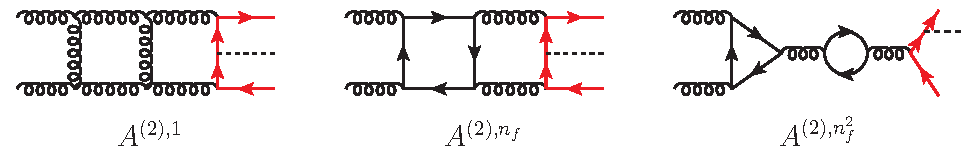
\includegraphics[width=0.95\textwidth]{ggbbH_amps_2L}
  \end{center}
  \caption{Sample Feynman diagrams corresponding to the various closed fermion loop contributions at two loops as specified in Eq.~\ref{eq:NfDecomposition2L}. 
  Black-dashed, red, black-spiralled and black lines represent Higgs bosons, bottom quarks, gluons and light quarks (bottom quarks included), respectively.}
  \label{fig:amp2L}
\end{figure}

The pole structure of the unrenormalised amplitudes in the HV scheme at one and two loops is given by~\cite{Catani:1998bh,Becher:2009qa,Becher:2009cu,Gardi:2009qi}:
\begin{align}
P^{(1)} & = 2 I^{(1)}(\eps) + \frac{\beta_0}{\eps} - 2 s_1,  
\label{eq:poles1L} \\
P^{(2)} & =   2 I^{(1)}(\eps) \bigg( \hat{A}^{(1)} - \frac{\beta_0}{\eps} + 2 s_1\bigg) + 4 I^{(2)}(\eps)
                + \bigg(\frac{2\beta_0}{\eps}-2 s_1\bigg) \hat{A}^{(1)} \nn 
& \hspace{0.4cm} - \frac{\beta_0^2}{\eps^2} + \frac{\beta_1}{2\eps} - 4 s_2 + \frac{2 s_1\beta_0}{\eps} \,,
\label{eq:poles2L}
\end{align}
where $\hat{A}^{(1)}$ is the unrenormalised one-loop amplitude normalised to the tree-level amplitude.
$s_1$ and $s_2$ are the bottom-quark Yukawa renormalisation constants, and their expressions can be found in Appendix~\ref{app:renormconstants}.
We used a mixed renormalisation scheme where the strong coupling $\alpha_s$ and the bottom-Yukawa coupling $y_b$ are renormalised in the $\overline{\text{MS}}$ scheme, while the bottom-quark mass and wave function are renormalised in the on-shell ($\mathrm{OS}$) scheme. This allows to keep $y_b$ finite while taking the bottom-quark mass smoothly to zero ($m_b^{\mathrm{OS}}\rightarrow 0$)~\cite{Mondini:2021nck}.
Such a mixed renormalisation scheme can be used so long as pure QCD corrections are considered. In fact, using the $\overline{\text{MS}}$ scheme to renormalise $y_b$ allows us to better control the convergence of the perturbative corrections by resumming the large logarithms that appear in the OS scheme by running $y_b$ to a scale close to the Higgs mass. In the presence of electroweak (EW) corrections, however, the relationship between
$y_b$ and $m_b$ must be imposed to guarantee the cancellation of UV singularities~\cite{Pagani:2020rsg}.


The $I^{(2)}(\eps)$ operator is defined by:
\begin{equation}
I^{(2)}(\eps) =   - \frac{1}{2}I^{(1)}(\eps) \left[ I^{(1)}(\eps)
              + \frac{\beta_0}{\eps} \right]
              + \frac{N(\eps)}{N(2\eps)} \left[ \frac{\beta_0}{2\eps}
                        + \frac{\gamma_{1}^{\cusp}}{8} \right] I^{(1)}(2\eps)
              + H^{(2)}(\eps) \,,
\end{equation}
while the $I^{(1)}(\eps)$ operators for $\bbh$ production in both the $gg$ and the $q\bar{q}$ channels are given at leading colour by:
\begin{align}
I_{\bbqqh}^{(1)}(\eps) &= -N_c \frac{N(\eps)}{2} \bigg( \frac{1}{\eps^2} + \frac{3}{2\eps} \bigg) \big[ \left(-s_{23}\right)^{-\eps} + \left(-s_{14}\right)^{-\eps} \big], 
\label{eq:I1bbqqh}\\
I_{\bbggh}^{(1)}(\eps) &= -N_c \frac{N(\eps)}{2} \bigg\lbrace \bigg( \frac{1}{\eps^2} + \frac{3}{4\eps} + \frac{\beta_0}{4 N_c\eps} \bigg) \big[ \left(-s_{23}\right)^{-\eps} + \left(-s_{14}\right)^{-\eps} \big]
                 + \bigg( \frac{1}{\eps^2} + \frac{\beta_0}{2 N_c \eps} \bigg) \left(-s_{34}\right)^{-\eps} \bigg\rbrace \,,
\label{eq:I1bbggh}
\end{align}
where $N(\eps) = {\mathrm{e}^{\eps \gamma_E}}/{\Gamma(1-\eps)}$, $s_{14} = s_{23}-s_{15}-s_{45}+p_5^2$ and:
\begin{align}
H_{\bbqqh}^{(2)}(\eps) &= \frac{1}{16\eps} \bigg\lbrace 4 \gamma_1^q - \gamma_1^\cusp \gamma_0^q + \frac{\pi^2}{4} \beta_0 \gamma_0^\cusp C_F \bigg\rbrace \,, \label{eq:H2bbqqH} \\
H_{\bbggh}^{(2)}(\eps) &=  \frac{1}{16\eps} \bigg\lbrace 2\left(\gamma_1^q+\gamma_1^g\right)
                                                - \frac{1}{2}\gamma_1^\cusp \left(\gamma_0^q+\gamma_0^g\right)
                                                + \frac{\pi^2}{8} \beta_0 \gamma_0^\cusp \left(C_F+C_A\right) \bigg\rbrace \,. \label{eq:H2bbggH}
\end{align}
The $\beta$ function coefficients and anomalous dimensions are given in Appendix~\ref{app:renormconstants}, while in Appendix~\ref{app:polestructure} we provide an explicit derivation of the pole operators.

The finite remainder of the $L$-loop partial amplitude is obtained by subtracting the poles $P^{(L)}$ (which include both the UV and IR singularities) from the unrenormalised partial amplitude $A^{(L)}$ and setting $\eps$ to $0$:
\begin{equation}
F^{(L)} = \lim_{\eps \to 0} \left[ A^{(L)} - P^{(L)} A^{(0)} \right]\,.
\label{eq:finiteremainder}
\end{equation}
The partial finite remainders $F^{(L)}$ inherit from the partial amplitudes the decomposition in powers of $n_f$:
\begin{align}
& F^{(1)} = N_c F^{(1),1} + n_f F^{(1),n_f}  \,,  
\label{eq:NfDecomposition1LF} \\
& F^{(2)} = N_c^2 F^{(2),1} + N_c n_f F^{(2),n_f} + n_f^2 F^{(2),n_f^2}  \,.
\label{eq:NfDecomposition2LF}
\end{align}
The full finite remainders $\mathcal{F}^{(L)}$ are obtained from the partial ones $F^{(L)}$ through a colour decomposition analogous to that given in Eq.~\ref{eq:colourdecomposition} for the bare amplitudes:
\begin{align}
&\mathcal{F}^{(L)}(1_{\bar b},2_{b},3_{g},4_{g} ,5_{H}) = n^L g_s^2 y_b \bigg[ 
  (T^{a_3} T^{a_4})_{i_2}^{\;\;\bar i_1} \,  F^{(L)}(1_{\bar b},2_{b},3_{g},4_{g} ,5_{H}) + ( 3 \leftrightarrow 4 ) \bigg]\,, \nonumber\\
&\mathcal{F}^{(L)}(1_{\bar b},2_{b},3_{\bar{q}},4_{q} ,5_{H}) = n^L  g_s^2 y_b 
 \delta_{i_4}^{\;\;\bar i_1} \delta_{i_2}^{\;\;\bar i_3}  \,
  F^{(L)}(1_{\bar b},2_{b},3_{\bar{q}},4_{q} ,5_{H}) \,,  \label{eq:colourdecompositionF} \\
&\mathcal{F}^{(L)}(1_{\bar b},2_{b},3_{\bar{b}},4_{b} ,5_{H}) = n^L  g_s^2 y_b \bigg[
  \delta_{i_4}^{\;\;\bar i_1} \delta_{i_2}^{\;\;\bar i_3}  \, \biggl( F^{(L)}(1_{\bar b},2_{b},3_{\bar{q}},4_{q} ,5_{H}) + F^{(L)}(3_{\bar b},4_{b},1_{\bar{q}},2_{q} ,5_{H}) \biggr) \,  \nonumber\\
& \hspace{4.5cm} -\delta_{i_2}^{\;\;\bar i_1} \delta_{i_4}^{\;\;\bar i_3}  \, \biggl( F^{(L)}(1_{\bar b},4_{b},3_{\bar{q}},2_{q} ,5_{H}) + F^{(L)}(3_{\bar b},2_{b},1_{\bar{q}},4_{q} ,5_{H}) \biggr) \bigg]\,.
\nonumber 
\end{align}


\subsection{Tree-Level Amplitudes}
\label{Hbbsec:trees}
The tree-level amplitudes can be obtained using the BCFW recursion relations~\cite{Britto:2004ap,Britto:2005fq} within the spinor helicity formalism. In the $\bar{b}bggH$ case, we choose to shift the momenta of gluons $3$ and $4$, while in the $\bar{b}b\bar{q}qH$ case we choose particles $1$ and $4$ to avoid shifting the momenta of adjacent quarks of the same flavour. Moreover, we ensure that the shifted brackets $[\hat{i}\ra, |\hat{j}]$ do not belong to particles of helicities $i^-, j^+$. These choices are necessary for the validity of the recursion relations as they prevent the shifted amplitude from having poles at infinity.

For the $\bar{b} b g g H$ channel we obtain the following non-vanishing tree-level amplitudes:
\begin{align} \label{eq:A0bbggh}
	A^{(0)}(1^+_{\bar{b}},2^+_{b},3^+_g,4^+_g,5_{H}) &=  \frac{s_5}{\spA 23 \spA 34 \spA 41} \,, \\
	A^{(0)}(1^+_{\bar{b}},2^+_{b},3^-_g,4^-_g,5_{H}) &= -\frac{\spB 12^2}{\spB 23\spB 34\spB 41} \,, \\
	A^{(0)}(1^+_{\bar{b}},2^+_{b},3^+_g,4^-_g,5_{H}) &= \frac{\spA 24 \spAB 451^2}{s_{234} \spA 23 \spA 34 \spAB 251}-\frac{s_5 \spB 13^3}{s_{134} \spB 14 \spB 34 \spAB 251} \,.
\end{align}
The $\bar{b},b$ quarks need to have the same helicity as that is the only way they can couple to the Higgs boson. 
For the $\bar{b} b \bar{q} q H$ channel the `all-plus' and MHV configurations vanish, and we are left with:
\begin{align} \label{eq:A0bbqqh}
	A^{(0)}(1^+_{\bar b},2^+_{b},3^+_{\bar q},4^-_{q},5_{H}) &=  \frac{\spAB 451^2}{s_{234} \spA 34 \spAB 251}+\frac{s_5 \spB 31^2}{s_{134} \spB 34 \spAB 251} \,. 
\end{align}

In both cases, due to the colour decomposition of the full amplitudes given by Eq.~\ref{eq:colourdecomposition}, the $A^{(0)}(1^+,2^+,3^-,4^+,5_{H})$ partial amplitude is related to $A^{(0)}(1^+,2^+,3^+,4^-,5_{H})$ by swapping the particles $1\leftrightarrow 2,3\leftrightarrow 4$ , and flipping the overall sign for the subprocess $\bbggh$. The remaining non-vanishing helicity configurations can be obtained by parity transformations, that is by swapping the brackets $\la ij \ra \leftrightarrow [ji]$.

\section{Amplitude Reduction and Reconstruction}
\label{Hbbsec:reduction}

To obtain the analytic form of the two-loop QCD helicity amplitudes, we employ the framework thoroughly discussed in Chapter~\ref{sec:tools}. Here, we provide a brief outline of it and supply process-specific details. We start by generating a set of Feynman diagrams contributing to 
both the $\bbggh$ and $\bbqqh$ processes using \texttt{QGRAF}~\cite{Nogueira:1991ex}, and perform diagram filtering, topology identification and colour decomposition using a collection of in-house \texttt{Mathematica} and \texttt{Form}~\cite{Kuipers:2012rf,Ruijl:2017dtg} scripts.  In the leading colour approximation, there are 749 (264) Feynman diagrams contributing to the two-loop $\bbggh$ ($\bbqqh$) QCD amplitudes, including all closed fermion loop contributions. The numerators of the loop amplitudes are then computed for each independent helicity configuration, and the spinor-helicity manipulations are carried out using the library \texttt{Spinney}~\cite{Cullen:2010jv}. The helicity dependent loop numerators are written in terms of spinor products ($\spA{i}{j}$, $\spB{i}{j}$), scalar products ($p_i\cdot p_j$, $k_i\cdot k_j$, $k_i \cdot p_j$) and spinor strings ($\spAB{i}{k_i}{j}$, $\spAB{i}{p_5}{j}$, $\spAA{i}{k_i p_5}{j}$, $\spBB{i}{k_i p_5}{j}$), where $p_i$'s and $k_i$'s are the external and loop momenta, respectively. The numerators are therefore expressed as linear combinations of monomials of loop-momentum dependent objects that multiply coefficients which depend only on the external kinematics.
As explained in Section~\ref{sec:MTs}, the coefficients are built from spinor products and strings (free of $k_i$) which not only are not independent, but are also incompatible with finite field arithmetic.

Both of these problems are solved by using MTs. To obtain a configuration for the off-shell five-particle configuration we begin with a massless configuration for six particles. While the exact parametrisation is not important, the form presented in Ref.~\cite{Badger:2016uuq} is a useful starting point. We can think of the massless process as the result of the off-shell leg decaying into a pair of massless particles. There are $3n-10 = 8$ independent variables in the six-particle process, but we can reduce the degrees of freedom by choosing one of the decay direction to be collinear with one of the other massless legs in the five-point kinematics. Since the MTs are associated with complex momenta, we consider the angle and square bracket spinors products to be independent. We can write this explicitly as follows: the six massless momenta $q_i^\mu$ are related to the off-shell five particle momenta $p_i^\mu$ by:
\begin{align}
  p_1^\mu = q_1^\mu\,, \ \qquad 
  p_2^\mu = q_2^\mu\,, \ \qquad 
  p_3^\mu = q_3^\mu\,, \ \qquad
  p_4^\mu = q_4^\mu \,, \ \qquad
  p_5^\mu = q_5^\mu+q_6^\mu \,.
\end{align}
We impose the constraints $\spA{q_2}{q_6} = 0 $ and $\spB{q_2}{q_6} = 0$ to reduce the independent variables to 6. 
We then apply a transformation onto the following choice of variables:
\begin{equation}
\begin{aligned}
  x_1 &= s_{12}, \\
  x_2 &= -\frac{\trp(1234)}{s_{12}s_{34}}, \\
  x_3 &= \frac{\trp(134152)}{s_{13}\trp{(1452)}}, \\
  x_4 &= \frac{s_{23}}{s_{12}}, \\
  x_5 &= -\frac{\trm(1(2+3)(1+5)523)}{s_{23}\trm(1523)}, \\
  x_6 &= \frac{s_{45}}{s_{12}},
\end{aligned}
\label{eq:mtvardefs}
\end{equation}
where $\tr_{\pm}(ij \cdots kl) = \frac{1}{2} \tr((1\pm\gamma_5)\slashed{p}_i\slashed{p}_j \cdots\slashed{p}_k\slashed{p}_l)$.
Some features of this parametrisation are particularly convenient. For example, the only dimensionful 
quantity is $x_1$, and $\tr_5$ is rational. However, such a choice does break some symmetries
in the problem and so different helicity configurations will have different complexities. For the
process considered here, the complexity was manageable using this form.
Applications to other off-shell five-particle processes may require further thought. 

Having set up a rational parametrisation of the external kinematics, the helicity dependent loop numerators are constructed analytically and
ready to be further processed.
This is the starting point of our numerical algorithm in the finite field setup. 
In order to write the amplitude in terms of scalar integrals, 
we first define the integral families for the 15 maximal topologies, which are shown in Fig.~\ref{fig:Hbbmaxtopos}. 
Each diagram topology appearing in the amplitude can be mapped onto at least one of them. 
After that is done, the objects which depend on the loop momenta in the numerators are written in terms of 
the 11 propagators and ISPs associated with the chosen maximal topology. 
These mapping procedures are performed numerically within the \texttt{FiniteFlow} framework~\cite{Peraro:2019svx}. 
We remark that since the maximal topologies have five external momenta, they completely span the 4-dimensional space and there is no need to introduce the spurious vectors. Thus, the integrand reduction technique of Section~\ref{sec:reduction} does not lead to an explicit dependence on $\eps$ into the numerators. Therefore, the coefficients of these scalar integrals are functions of the external kinematics only, in the form of MTs.
\begin{figure}
    \centering
    \begin{subfigure}{0.3\linewidth}
    \scalebox{0.8}{
		\begin{tikzpicture}
			\begin{feynman}[small]
				\vertex (v1);
				\vertex[above left=0.8cm of v1] (i1) {$p_1$};
				\vertex[right = of v1] (v2);
				\vertex[yshift=0.3cm, right = 0.8cm of v2] (v3);
				\vertex[above right = 0.8cm of v3] (f1) {$p_5$};			
				
				\vertex[below = of v1] (v7) ;
				\vertex[below left = 0.8cm of v7] (i2) {$p_4$};
				\vertex[right = of v7] (v6) ;
				\vertex[yshift=-0.3cm, right = 0.8cm of v6] (v5) ;
				\vertex[below right = 0.8cm of v5] (f3) {$p_3$};
				
				\vertex[xshift=0.6cm, yshift=0.2cm, below = of v3] (v4);
				\vertex[right = 0.8cm of v4] (f2) {$p_2$};
				
				\diagram*{
					(i1) -- (v1) -- (v2) -- (v3) -- (v4) -- (v5),
					(i2) -- (v7) -- (v6) -- (v5),
					(v3) -- [scalar, very thick] (f1),
					(v4) -- (f2),
					(v5) -- (f3),
					(v1) -- (v7),
					(v2) -- (v6),
				};
			\end{feynman}
		\end{tikzpicture}
    }
    \end{subfigure}
    \begin{subfigure}{0.3\linewidth}
    \scalebox{0.8}{
		\begin{tikzpicture}
			\begin{feynman}[small]
				\vertex (v1);
				\vertex[above left=0.8cm of v1] (i1) {$p_2$};
				\vertex[right = of v1] (v2);
				\vertex[yshift=0.3cm, right = 0.8cm of v2] (v3);
				\vertex[above right = 0.8cm of v3] (f1) {$p_5$};			
				
				\vertex[below = of v1] (v7) ;
				\vertex[below left = 0.8cm of v7] (i2) {$p_3$};
				\vertex[right = of v7] (v6) ;
				\vertex[yshift=-0.3cm, right = 0.8cm of v6] (v5) ;
				\vertex[below right = 0.8cm of v5] (f3) {$p_4$};
				
				\vertex[xshift=0.6cm, yshift=0.2cm, below = of v3] (v4);
				\vertex[right = 0.8cm of v4] (f2) {$p_1$};
				
				\diagram*{
					(i1) -- (v1) -- (v2) -- (v3) -- (v4) -- (v5),
					(i2) -- (v7) -- (v6) -- (v5),
					(v3) -- [scalar, very thick] (f1),
					(v4) -- (f2),
					(v5) -- (f3),
					(v1) -- (v7),
					(v2) -- (v6),
				};
			\end{feynman}
		\end{tikzpicture}
    }
    \end{subfigure}
    \begin{subfigure}{0.3\linewidth}
    \scalebox{0.8}{
		\begin{tikzpicture}
			\begin{feynman}[small]
				\vertex (v1);
				\vertex[above left=0.8cm of v1] (i1) {$p_4$};
				\vertex[right = of v1] (v2);
				\vertex[yshift=0.3cm, right = 0.8cm of v2] (v3);
				\vertex[above right = 0.8cm of v3] (f1) {$p_1$};			
				
				\vertex[below = of v1] (v7) ;
				\vertex[below left = 0.8cm of v7] (i2) {$p_3$};
				\vertex[right = of v7] (v6) ;
				\vertex[yshift=-0.3cm, right = 0.8cm of v6] (v5) ;
				\vertex[below right = 0.8cm of v5] (f3) {$p_2$};
				
				\vertex[xshift=0.6cm, yshift=0.2cm, below = of v3] (v4);
				\vertex[right = 0.8cm of v4] (f2) {$p_5$};
				
				\diagram*{
					(i1) -- (v1) -- (v2) -- (v3) -- (v4) -- (v5),
					(i2) -- (v7) -- (v6) -- (v5),
					(v3) -- (f1),
					(v4) -- [scalar, very thick] (f2),
					(v5) -- (f3),
					(v1) -- (v7),
					(v2) -- (v6),
				};
			\end{feynman}
		\end{tikzpicture}
    }
    \end{subfigure}
    \begin{subfigure}{0.3\linewidth}
    \scalebox{0.8}{
		\begin{tikzpicture}
			\begin{feynman}[small]
				\vertex (v1);
				\vertex[above left=0.8cm of v1] (i1) {$p_5$};
				\vertex[right = of v1] (v2);
				\vertex[yshift=0.3cm, right = 0.8cm of v2] (v3);
				\vertex[above right = 0.8cm of v3] (f1) {$p_1$};			
				
				\vertex[below = of v1] (v7) ;
				\vertex[below left = 0.8cm of v7] (i2) {$p_2$};
				\vertex[right = of v7] (v6) ;
				\vertex[yshift=-0.3cm, right = 0.8cm of v6] (v5) ;
				\vertex[below right = 0.8cm of v5] (f3) {$p_3$};
				
				\vertex[xshift=0.6cm, yshift=0.2cm, below = of v3] (v4);
				\vertex[right = 0.8cm of v4] (f2) {$p_4$};
				
				\diagram*{
					(i1) -- [scalar, very thick] (v1) -- (v2) -- (v3) -- (v4) -- (v5),
					(i2) -- (v7) -- (v6) -- (v5),
					(v3) -- (f1),
					(v4) -- (f2),
					(v5) -- (f3),
					(v1) -- (v7),
					(v2) -- (v6),
				};
			\end{feynman}
		\end{tikzpicture}
    }
    \end{subfigure}
    \begin{subfigure}{0.3\linewidth}
    \scalebox{0.8}{
		\begin{tikzpicture}
			\begin{feynman}[small]
				\vertex (v1);
				\vertex[above left=0.8cm of v1] (i1) {$p_5$};
				\vertex[right = of v1] (v2);
				\vertex[yshift=0.3cm, right = 0.8cm of v2] (v3);
				\vertex[above right = 0.8cm of v3] (f1) {$p_2$};			
				
				\vertex[below = of v1] (v7) ;
				\vertex[below left = 0.8cm of v7] (i2) {$p_1$};
				\vertex[right = of v7] (v6) ;
				\vertex[yshift=-0.3cm, right = 0.8cm of v6] (v5) ;
				\vertex[below right = 0.8cm of v5] (f3) {$p_4$};
				
				\vertex[xshift=0.6cm, yshift=0.2cm, below = of v3] (v4);
				\vertex[right = 0.8cm of v4] (f2) {$p_3$};
				
				\diagram*{
					(i1) -- [scalar, very thick] (v1) -- (v2) -- (v3) -- (v4) -- (v5),
					(i2) -- (v7) -- (v6) -- (v5),
					(v3) -- (f1),
					(v4) -- (f2),
					(v5) -- (f3),
					(v1) -- (v7),
					(v2) -- (v6),
				};
			\end{feynman}
		\end{tikzpicture}
    }
    \end{subfigure}
    \begin{subfigure}{0.3\linewidth}
    \scalebox{0.8}{
		\begin{tikzpicture}
			\begin{feynman}[small]
				\vertex (v1);
				\vertex[left = 0.8cm of v1] (i1) {$p_1$};
				\vertex[above right =1cm of v1] (v2);
				\vertex[below right =1cm of v1] (v3);				
				\vertex[yshift=0.3cm, right = 0.7cm of v2] (v4);	
				\vertex[yshift=-0.6cm, right = 0.7cm of v4] (v5);
				\vertex[yshift=-0.3cm, right = 0.7cm of v3] (v7);
				\vertex[yshift=0.6cm, right = 0.7cm of v7] (v6);	
				\vertex[above right = 0.8cm of v4] (i2) {$p_5$};
				\vertex[yshift=0.2cm, right = 0.8cm of v5] (i3) {$p_2$};
				\vertex[yshift=-0.2cm, right = 0.8cm of v6] (i4) {$p_3$};
				\vertex[below right = 0.8cm of v7] (i5) {$p_4$};
				
				\diagram*{
					(i1) -- (v1) -- (v2) -- (v3) -- (v1),
					(v2) -- (v4) -- (v5) -- (v6) -- (v7) -- (v3),
					(v4) -- [scalar, very thick] (i2),
					(v5) -- (i3),
					(v6) -- (i4),
					(v7) -- (i5),
				};
			\end{feynman}
		\end{tikzpicture}
    }
    \end{subfigure}
    \begin{subfigure}{0.3\linewidth}
    \scalebox{0.8}{
		\begin{tikzpicture}
			\begin{feynman}[small]
				\vertex (v1);
				\vertex[left = 0.8cm of v1] (i1) {$p_2$};
				\vertex[above right =1cm of v1] (v2);
				\vertex[below right =1cm of v1] (v3);				
				\vertex[yshift=0.3cm, right = 0.7cm of v2] (v4);	
				\vertex[yshift=-0.6cm, right = 0.7cm of v4] (v5);
				\vertex[yshift=-0.3cm, right = 0.7cm of v3] (v7);
				\vertex[yshift=0.6cm, right = 0.7cm of v7] (v6);	
				\vertex[above right = 0.8cm of v4] (i2) {$p_5$};
				\vertex[yshift=0.2cm, right = 0.8cm of v5] (i3) {$p_1$};
				\vertex[yshift=-0.2cm, right = 0.8cm of v6] (i4) {$p_4$};
				\vertex[below right = 0.8cm of v7] (i5) {$p_3$};
				
				\diagram*{
					(i1) -- (v1) -- (v2) -- (v3) -- (v1),
					(v2) -- (v4) -- (v5) -- (v6) -- (v7) -- (v3),
					(v4) -- [scalar, very thick] (i2),
					(v5) -- (i3),
					(v6) -- (i4),
					(v7) -- (i5),
				};
			\end{feynman}
		\end{tikzpicture}
    }
    \end{subfigure}
    \begin{subfigure}{0.3\linewidth}
    \scalebox{0.8}{
		\begin{tikzpicture}
			\begin{feynman}[small]
				\vertex (v1);
				\vertex[left = 0.8cm of v1] (i1) {$p_4$};
				\vertex[above right =1cm of v1] (v2);
				\vertex[below right =1cm of v1] (v3);				
				\vertex[yshift=0.3cm, right = 0.7cm of v2] (v4);	
				\vertex[yshift=-0.6cm, right = 0.7cm of v4] (v5);
				\vertex[yshift=-0.3cm, right = 0.7cm of v3] (v7);
				\vertex[yshift=0.6cm, right = 0.7cm of v7] (v6);	
				\vertex[above right = 0.8cm of v4] (i2) {$p_1$};
				\vertex[yshift=0.2cm, right = 0.8cm of v5] (i3) {$p_5$};
				\vertex[yshift=-0.2cm, right = 0.8cm of v6] (i4) {$p_2$};
				\vertex[below right = 0.8cm of v7] (i5) {$p_3$};
				
				\diagram*{
					(i1) -- (v1) -- (v2) -- (v3) -- (v1),
					(v2) -- (v4) -- (v5) -- (v6) -- (v7) -- (v3),
					(v4) -- (i2),
					(v5) -- [scalar, very thick] (i3),
					(v6) -- (i4),
					(v7) -- (i5),
				};
			\end{feynman}
		\end{tikzpicture}
    }
    \end{subfigure}
    \begin{subfigure}{0.3\linewidth}
    \scalebox{0.8}{
		\begin{tikzpicture}
			\begin{feynman}[small]
				\vertex (v1);
				\vertex[left = 0.8cm of v1] (i1) {$p_3$};
				\vertex[above right =1cm of v1] (v2);
				\vertex[below right =1cm of v1] (v3);				
				\vertex[yshift=0.3cm, right = 0.7cm of v2] (v4);	
				\vertex[yshift=-0.6cm, right = 0.7cm of v4] (v5);
				\vertex[yshift=-0.3cm, right = 0.7cm of v3] (v7);
				\vertex[yshift=0.6cm, right = 0.7cm of v7] (v6);	
				\vertex[above right = 0.8cm of v4] (i2) {$p_2$};
				\vertex[yshift=0.2cm, right = 0.8cm of v5] (i3) {$p_5$};
				\vertex[yshift=-0.2cm, right = 0.8cm of v6] (i4) {$p_1$};
				\vertex[below right = 0.8cm of v7] (i5) {$p_4$};
				
				\diagram*{
					(i1) -- (v1) -- (v2) -- (v3) -- (v1),
					(v2) -- (v4) -- (v5) -- (v6) -- (v7) -- (v3),
					(v4) -- (i2),
					(v5) -- [scalar, very thick] (i3),
					(v6) -- (i4),
					(v7) -- (i5),
				};
			\end{feynman}
		\end{tikzpicture}
    }
    \end{subfigure}
    \begin{subfigure}{0.3\linewidth}
    \scalebox{0.8}{
		\begin{tikzpicture}
			\begin{feynman}[small]
				\vertex (v1);
				\vertex[left = 0.8cm of v1] (i1) {$p_5$};
				\vertex[above right =1cm of v1] (v2);
				\vertex[below right =1cm of v1] (v3);				
				\vertex[yshift=0.3cm, right = 0.7cm of v2] (v4);	
				\vertex[yshift=-0.6cm, right = 0.7cm of v4] (v5);
				\vertex[yshift=-0.3cm, right = 0.7cm of v3] (v7);
				\vertex[yshift=0.6cm, right = 0.7cm of v7] (v6);	
				\vertex[above right = 0.8cm of v4] (i2) {$p_2$};
				\vertex[yshift=0.2cm, right = 0.8cm of v5] (i3) {$p_3$};
				\vertex[yshift=-0.2cm, right = 0.8cm of v6] (i4) {$p_4$};
				\vertex[below right = 0.8cm of v7] (i5) {$p_1$};
				
				\diagram*{
					(i1) -- [scalar, very thick] (v1) -- (v2) -- (v3) -- (v1),
					(v2) -- (v4) -- (v5) -- (v6) -- (v7) -- (v3),
					(v4) -- (i2),
					(v5) -- (i3),
					(v6) -- (i4),
					(v7) -- (i5),
				};
			\end{feynman}
		\end{tikzpicture}
    }
    \end{subfigure}
    \begin{subfigure}{0.3\linewidth}
    \scalebox{0.8}{
		\begin{tikzpicture}\hspace{0.5cm}
			\begin{feynman}[small]
				\vertex (v1);
				\vertex[yshift=0.2cm, right =1cm of v1] (v2);
				\vertex[xshift=0.7cm, below =1cm of v2] (v3);				
				\vertex[below = 1.5cm of v1] (v5);
				\vertex[yshift=-0.2cm, right =1cm of v5] (v4);
				\vertex[below=0.3cm of v1] (v6);
				\vertex[below=0.9cm of v6] (v7);
				
				\vertex[above left = 0.8cm of v1] (i1) {$p_5$};
				\vertex[above right = 0.8cm of v2] (i2) {$p_2$};
				\vertex[right = 0.8cm of v3] (i3) {$p_3$};
				\vertex[below right = 0.8cm of v4] (i4) {$p_4$};
				\vertex[below left = 0.8cm of v5] (i5) {$p_1$};
				
				\draw ([yshift=-0.75cm]v1) circle (0.45cm);
				
				\diagram*{
					(v6) -- (v1) -- (v2) -- (v3) -- (v4) -- (v5) -- (v7), 
					(v1) -- [scalar, very thick] (i1),
					(v2) -- (i2),
					(v3) -- (i3),
					(v4) -- (i4),
					(v5) -- (i5),
					
				};
			\end{feynman}
		\end{tikzpicture}
    }
    \end{subfigure}
    \begin{subfigure}{0.3\linewidth}
    \scalebox{0.8}{
		\begin{tikzpicture}\hspace{0.5cm}
			\begin{feynman}[small]
				\vertex (v1);
				\vertex[yshift=0.2cm, right =1cm of v1] (v2);
				\vertex[xshift=0.7cm, below =1cm of v2] (v3);				
				\vertex[below = 1.5cm of v1] (v5);
				\vertex[yshift=-0.2cm, right =1cm of v5] (v4);
				\vertex[below=0.3cm of v1] (v6);
				\vertex[below=0.9cm of v6] (v7);
				
				\vertex[above left = 0.8cm of v1] (i1) {$p_5$};
				\vertex[above right = 0.8cm of v2] (i2) {$p_1$};
				\vertex[right = 0.8cm of v3] (i3) {$p_4$};
				\vertex[below right = 0.8cm of v4] (i4) {$p_3$};
				\vertex[below left = 0.8cm of v5] (i5) {$p_2$};
				
				\draw ([yshift=-0.75cm]v1) circle (0.45cm);
				
				\diagram*{
					(v6) -- (v1) -- (v2) -- (v3) -- (v4) -- (v5) -- (v7), 
					(v1) -- [scalar, very thick] (i1),
					(v2) -- (i2),
					(v3) -- (i3),
					(v4) -- (i4),
					(v5) -- (i5),
					
				};
			\end{feynman}
		\end{tikzpicture}
    }
    \end{subfigure}
    \begin{subfigure}{0.3\linewidth}
    \scalebox{0.8}{
		\begin{tikzpicture}\hspace{0.5cm}
			\begin{feynman}[small]
				\vertex (v1);
				\vertex[yshift=0.2cm, right =1cm of v1] (v2);
				\vertex[xshift=0.7cm, below =1cm of v2] (v3);				
				\vertex[below = 1.5cm of v1] (v5);
				\vertex[yshift=-0.2cm, right =1cm of v5] (v4);
				\vertex[below=0.3cm of v1] (v6);
				\vertex[below=0.9cm of v6] (v7);
				
				\vertex[above left = 0.8cm of v1] (i1) {$p_1$};
				\vertex[above right = 0.8cm of v2] (i2) {$p_5$};
				\vertex[right = 0.8cm of v3] (i3) {$p_2$};
				\vertex[below right = 0.8cm of v4] (i4) {$p_3$};
				\vertex[below left = 0.8cm of v5] (i5) {$p_4$};
				
				\draw ([yshift=-0.75cm]v1) circle (0.45cm);
				
				\diagram*{
					(v6) -- (v1) -- (v2) -- (v3) -- (v4) -- (v5) -- (v7), 
					(v1) -- (i1),
					(v2) -- [scalar, very thick] (i2),
					(v3) -- (i3),
					(v4) -- (i4),
					(v5) -- (i5),
					
				};
			\end{feynman}
		\end{tikzpicture}
    }
    \end{subfigure}
    \begin{subfigure}{0.3\linewidth}
    \scalebox{0.8}{
		\begin{tikzpicture}\hspace{0.5cm}
			\begin{feynman}[small]
				\vertex (v1);
				\vertex[yshift=0.2cm, right =1cm of v1] (v2);
				\vertex[xshift=0.7cm, below =1cm of v2] (v3);				
				\vertex[below = 1.5cm of v1] (v5);
				\vertex[yshift=-0.2cm, right =1cm of v5] (v4);
				\vertex[below=0.3cm of v1] (v6);
				\vertex[below=0.9cm of v6] (v7);
				
				\vertex[above left = 0.8cm of v1] (i1) {$p_2$};
				\vertex[above right = 0.8cm of v2] (i2) {$p_5$};
				\vertex[right = 0.8cm of v3] (i3) {$p_1$};
				\vertex[below right = 0.8cm of v4] (i4) {$p_4$};
				\vertex[below left = 0.8cm of v5] (i5) {$p_3$};
				
				\draw ([yshift=-0.75cm]v1) circle (0.45cm);
				
				\diagram*{
					(v6) -- (v1) -- (v2) -- (v3) -- (v4) -- (v5) -- (v7), 
					(v1) -- (i1),
					(v2) -- [scalar, very thick] (i2),
					(v3) -- (i3),
					(v4) -- (i4),
					(v5) -- (i5),
					
				};
			\end{feynman}
		\end{tikzpicture}
        }
    \end{subfigure}
    \begin{subfigure}{0.3\linewidth}
        \scalebox{0.8}{
		\begin{tikzpicture}\hspace{0.5cm}
			\begin{feynman}[small]
				\vertex (v1);
				\vertex[yshift=0.2cm, right =1cm of v1] (v2);
				\vertex[xshift=0.7cm, below =1cm of v2] (v3);				
				\vertex[below = 1.5cm of v1] (v5);
				\vertex[yshift=-0.2cm, right =1cm of v5] (v4);
				\vertex[below=0.3cm of v1] (v6);
				\vertex[below=0.9cm of v6] (v7);
				
				\vertex[above left = 0.8cm of v1] (i1) {$p_4$};
				\vertex[above right = 0.8cm of v2] (i2) {$p_1$};
				\vertex[right = 0.8cm of v3] (i3) {$p_5$};
				\vertex[below right = 0.8cm of v4] (i4) {$p_2$};
				\vertex[below left = 0.8cm of v5] (i5) {$p_3$};
				
				\draw ([yshift=-0.75cm]v1) circle (0.45cm);
				
				\diagram*{
					(v6) -- (v1) -- (v2) -- (v3) -- (v4) -- (v5) -- (v7), 
					(v1) -- (i1),
					(v2) -- (i2),
					(v3) -- [scalar, very thick] (i3),
					(v4) -- (i4),
					(v5) -- (i5),
					
				};
			\end{feynman}
		\end{tikzpicture}
        }
    \end{subfigure}
    \caption{Maximal topologies present in the computation of the two-loop $\ppbbh$ amplitudes. They were previously also used in Ref.~\cite{Badger:2021nhg}. The massive particle is marked with a bold dashed line.}
    \label{fig:Hbbmaxtopos}
\end{figure}

At this stage, the loop amplitude is expressed as a linear combination of scalar integrals that can be reduced to a set of MIs using the IBP reduction method~\cite{Chetyrkin:1981qh} within the finite field setup. The IBP relations are generated using \texttt{LiteRed}~\cite{Lee:2012cn} and solved numerically over finite fields using the Laporta algorithm~\cite{Laporta:2001dd}. The IBP reduction is performed directly to a set of MIs with UT weight identified in Ref.~\cite{Abreu:2020jxa}. The UT MIs are further expanded onto a basis of special functions $f$ that is built out of the MI components, as proposed in Ref.~\cite{Badger:2021nhg}. We refer to this basis of special functions as the \textit{master integral function basis}.
Subtracting the UV and IR poles from the bare helicity amplitudes and performing Laurent expansion in the dimensional regulator $\eps$, we arrive at the following expression for the finite remainders:
\begin{equation}
F^{(L)} = \sum_{i} r_i(x) m_i(f)\,,
\label{eq:finrem}
\end{equation}
where $m_i(f)$ are monomials of the special functions and $r_i$ are rational functions of the MTs $x$. It is important to note that the UT MIs involves three square roots. One is related to the pseudo-scalar invariant $\tr_5$, which captures the parity-odd part of the spinor expressions and is therefore present already in the rational coefficients. This square root is rationalised by the MT-inspired parametrisation, Eq.~\ref{eq:mtvardefs}. The other two square roots are associated with the three-mass triangle Gram determinants:
\begin{align}
  \Delta_3^{(1)} &= 2 \sqrt{(p_{23} \cdot p_{5})^2 - p_5^2 s_{23}} \,,&
  \Delta_3^{(2)} &= 2 \sqrt{(p_{12} \cdot p_{5})^2 - p_5^2 s_{12}} \,,
  \label{eq:squareroots}
\end{align}
where $p_{ij} = p_i + p_j$.
They are not rationalised by our parametrisation and may therefore be problematic for the finite field setup. We overcome this issue by absorbing the three square roots into the definition of the UT MIs, which is possible because they appear only as overall normalisations of the latter. As a result, they are contained in the monomials $m_i(f)$ in Eq.~\ref{eq:finrem} and do not appear in the amplitude reconstruction.
We note that in our computation, while the $\tr_5$ originating from the UT MIs is absorbed in $m_i(f)$, 
the $\tr_5$ already present in the coefficients is rationalised and present in the amplitude reconstruction.

At this stage, we have an algorithm which computes the coefficients of the special function monomials, $r_i(x)$ in Eq.~\ref{eq:squareroots}, 
numerically over finite fields for each of the independent helicity configurations of the two processes $\bar{b}bggH$ and $\bar{b}b\bar{q}qH$. 
We emphasise that from the start of our numerical algorithm until reaching $r_i(x)$, the computation is done within one system of \texttt{FiniteFlow} graphs.
The last step is the functional reconstruction of the rational coefficients. This task is made challenging by the high polynomial degrees, which are shown in the third column of Tables~\ref{tab:degrees2g2bH} and~\ref{tab:degrees2q2bH}. We tackle the complexity of the reconstruction through the strategy already used in Refs.~\cite{Badger:2021nhg,Badger:2021imn}. We refer to Ref.~\cite{Badger:2021imn} for a thorough discussion, and give here only a brief outline. 

The first step of the strategy consists in fitting the linear relations among the rational coefficients. These linear relations are then used to express the rational coefficients in terms of a set of linearly independent coefficients, which are chosen to have the lowest possible degrees. The degrees of the independent rational coefficients are given in the fourth column of Tables~\ref{tab:degrees2g2bH} and~\ref{tab:degrees2q2bH}.

The second step of our reconstruction strategy consists of determining the factors in the denominators of the rational coefficients. The analytic structure of the special functions is determined by a set of algebraic functions of the kinematics called letters. In other words, the singularities of the special functions and of their discontinuities are located on the hypersurfaces where any of the letters vanish (or go to infinity). It is therefore natural to expect that the rational coefficients which multiply the special functions should feature poles which are similarly linked to the letters, given for our process in Ref.~\cite{Abreu:2020jxa}. 
This motivates us to include the letters into an ansatz for the denominators of the coefficients. Since the helicity amplitudes also contain phase information, we must include spinor structures as well. It is then simple to check, on a univariate slice of the amplitude, whether the terms in the ansatz are present in the denominators or not. For our amplitudes, we find the following list to be sufficient:
\begin{equation}
\begin{aligned}
\biggl\{  & \spA{i}{j} \,,  \spB{i}{j}  \,, \spAB{i}{p_5}{j}  \,, s_{ij} \,, s_{ij} - s_{kl} \,, 
  s_{i5} - p_5^2 \,, p_5^2 \,, \tr_5 \, , \Delta_1 \,, \Delta_2 \, , \\
&  s_{15} (s_{13}+s_{34}) - p_5^2  s_{34}  \,,
 s_{25} (s_{24}+s_{34}) - p_5^2  s_{34} \biggr\} \,,
\end{aligned}
\label{eq:coeffansatz}
\end{equation}
where the indices $i,j$ in the spinor expressions vary from $1$ to $4$, while the indices $i,j,k,l$ in the Mandelstam invariants vary from $1$ to $5$. The various free indices in each of the factors are understood to be different from each other. Here, the ansatz of Eq.~\ref{eq:coeffansatz} allows us to determine the denominators entirely, as well as some factors in the numerators.

Having determined the denominators of the rational coefficients, we can proceed to the third and last step of our reconstruction strategy:  a univariate partial fraction decomposition `on the fly'. We find that, with the parameterisation of the external kinematics given by Eq.~\ref{eq:mtvardefs}, partial fractioning with respect to $x_5$ is the most convenient choice. 
The partial fraction decomposition of multivariate functions has recently drawn a lot interest as a powerful tool to simplify the analytic expressions of scattering amplitudes. A number of new approaches have been proposed, which make use of algebraic geometry techniques to handle the multivariate case efficiently~\cite{Leinartas:1978,Raichev:2012,Abreu:2019odu,Boehm:2020ijp,Heller:2021qkz}. However, these algorithms are applied to known \textit{analytic} expressions, i.e. after the rational reconstruction has been performed. On the contrary, our univariate partial fraction decomposition can be performed within the finite field setup itself, which consequently simplifies the reconstruction of the coefficients.
The algorithm makes use of the knowledge of the denominators to construct an ansatz for the decomposition into partial fractions with respect to the chosen variable. The coefficients of this ansatz can then be solved for and reconstructed. To this end, we perform a further matching of their factors against the ansatz in Eq.~\ref{eq:coeffansatz}. The matched factors are then removed, and the remaining functions are reconstructed with \texttt{FiniteFlow}'s reconstruction algorithm (see Section~\ref{sec:ratfuncs}). The degrees of the rational coefficients which remain to be reconstructed are shown in the fifth column of Tables~\ref{tab:degrees2g2bH} and~\ref{tab:degrees2q2bH}. Note that after partial fractioning, the denominators are not entirely determined from the ansatz in Eq.~\ref{eq:coeffansatz}. The univariate partial fraction decomposition in fact introduces spurious factors in the denominators. The latter could be determined as well, but we refrain from doing so as it does not reduce the complexity of the reconstruction.

\renewcommand{\arraystretch}{1.5}
\begin{table}[t!]
\centering
\begin{tabularx}{0.95\textwidth}{|C{0.8}|C{1.2}|C{0.8}|C{1.0}|C{1.2}|C{1.0}|}
\hline
 $\bbggh$     & helicity configurations & $r_i(x)$ & independent $r_i(x)$ & partial fraction in $x_5$ & number of points \\
\hline
$F^{(2),1}$ & $++++$ & 63/57   & 52/46   & 20/6  & 3361 \\
            & $+++-$ & 135/134 & 119/120 & 28/22 & 24901 \\
%            & $++-+$ & 120/116 & 110/107 & 28/16 & 19052 \\
            & $++--$ & 105/111 & 105/111 & 22/12 & 4797 \\
\hline
$F^{(2),n_f}$ & $++++$ & 45/41 & 45/41 & 16/6 & 1381 \\
              & $+++-$ & 94/95 & 94/95 & 17/6 & 1853 \\
%              & $++-+$ & 88/86 & 88/86 & 17/9 & 3329 \\
              & $++--$ & 89/95 & 62/69 & 18/3 & 2492 \\
\hline
$F^{(2),n_f^2}$ & $++++$ & 12/8  & 9/7   & 0/0 & 3 \\
                & $+++-$ & 11/16 & 11/16 & 3/0 & 22 \\
%                & $++-+$ & 12/13 & 12/13 & 3/0 & 22 \\
                & $++--$ & 12/20 & 8/16  & 8/0 & 242 \\
\hline
\end{tabularx}
\caption{\label{tab:degrees2g2bH} Maximum numerator/denominator polynomial degrees of the finite remainder coefficients $r_i(x)$ in Eq.~\ref{eq:finrem} 
at each stage of our reconstruction steps, together with the number of sample points needed for the analytic reconstruction in the $\bbggh$ subprocess, for the various closed fermion loop contributions.}
\end{table}

\begin{table}[t!]
\centering
\begin{tabularx}{0.95\textwidth}{|C{0.8}|C{1.2}|C{0.8}|C{1.0}|C{1.2}|C{1.0}|}
\hline
 $\bbqqh$     & helicity configurations & $r_i(x)$ & independent $r_i(x)$ & partial fraction in $x_5$ & number of points \\
\hline
$F^{(2),1}$ & $+++-$ & 82/81 & 69/70 & 24/16 & 10326 \\
%            & $++-+$ & 77/75 & 63/63 & 24/16 & 10326 \\
\hline
$F^{(2),n_f}$ & $+++-$ & 28/30 & 25/24 & 8/6 & 379 \\
%              & $++-+$ & 32/33 & 22/23 & 8/6 & 379 \\
\hline
$F^{(2),n_f^2}$ & $+++-$ & 6/11  & 6/11  & 3/0 & 22 \\
%                & $++-+$ & 10/12 & 10/12 & 3/0 & 22 \\
\hline
\end{tabularx}
\caption{\label{tab:degrees2q2bH} Maximum numerator/denominator polynomial degrees of the finite remainder coefficients $r_i(x)$ in Eq.~\ref{eq:finrem} 
at each stage of our reconstruction steps, together with the number of sample points needed for the analytic reconstruction in the $\bbqqh$ subprocess, for the various closed fermion loop contributions.}
\end{table}

Following the strategy outlined above, we reconstructed the partial finite remainders for the independent mostly-plus helicity configurations of the subprocesses $\bbggh$ and $\bbqqh$. The mostly-minus helicity finite remainders can be obtained by parity conjugation. Moreover, the finite remainders for the helicity configuration $++-+$ can be obtained by swapping $1\leftrightarrow2$, $3\leftrightarrow 4$ in the $+++-$ finite remainders, as discussed in Section~\ref{Hbbsec:trees} for the tree-level amplitudes. 
This symmetry follows from the colour structure and thus holds at any loop order. 
We could therefore evaluate the $++-+$ finite remainders by permuting numerically the $+++-$ ones, as we do in order to get all the other helicity configurations from the independent ones. By permuting numerically, we mean that we obtain the values of the permuted finite remainders by evaluating the unpermuted ones at permuted points. This is possible because our approach to the evaluation of the special functions, which we discuss in Section~\ref{Hbbsec:Hbasis}, handles the analytic continuation to any region automatically. Each numerical permutation therefore amounts to one more evaluation for each point. The permutation that takes from $+++-$ to $++-+$ is however peculiar, as it is covered by the basis of special functions defined in Ref.~\cite{Badger:2021nhg}. We can thus reconstruct the finite remainders for both helicity configurations directly in terms of the same basis of special functions. This is much more convenient, as it reduces the number of permutations which need to be carried out numerically, this way decreasing the global evaluation time of the finite remainders. For this reason we reconstructed the analytic expression of the $++-+$ finite remainders as well, and include the $++-+$ configuration in the independent helicity set in the following sections. 
The relation with the $+++-$ configuration constitutes a non-trivial check of our results, which we discuss in Section~\ref{Hbbsec:validation}.


\section[A Custom Basis for the Finite Remainders]{A Custom Basis of Special Functions for the Finite Remainders}

\label{Hbbsec:Hbasis}
The one and two-loop finite remainders are expressed as combinations of rational coefficients --- functions of the MTs Eq.~\ref{eq:mtvardefs} --- and monomials of square roots and elements of the MI function basis $\{f^{(w)}_i\}$. The latter were classified in Ref.~\cite{Badger:2021nhg} so as to span the cyclic permutations of the planar five-particle integrals with one massive off-shell leg up to two loops. The function space of the finite remainders is however simpler than that of the integrals and of the amplitudes. This becomes particularly clear when we express the special functions in terms of CIIs~\cite{Chen:1977oja}, which we have introduced in Section~\ref{sec:canonicalform}. Here, we will write the special functions as:
\begin{align} \label{eq:Chen}
\left[W_{i_1}, \ldots, W_{i_n}  \right]_{s_0} (s) = \int_0^1 dt \, \frac{d \log W_{i_n}\left(\gamma(t)\right)}{dt} \left[W_{i_1}, \ldots, W_{i_{n-1}}  \right]_{s_0} \left(\gamma(t)\right) \,,
\end{align}
where $\left\{ d\log W_i \right\}$ are the logarithmic integration kernels and their arguments $W_i$ are algebraic functions of the external kinematics. The cumulative dependence on external kinematics is denoted by $s$, while $s_0$ is an arbitrary reference point, and $\gamma$ is an arbitrary contour in the phase space going from $\gamma(0)=s_0$ to $\gamma(1)=s$. The iteration starts with $[]_{s_0}(s) := 1$. The transcendental weight of the special functions is then trivially given by $n$ in Eq.~\ref{eq:Chen}. At two loops up to order $\eps^0$ iterated integrals with transcendental weight up to four are required. In our case, the integration kernels are given by the letters $\{W_i\}$ of the alphabet defined in Ref.~\cite{Abreu:2020jxa}. 
Although they may look rather abstract, CIIs offer several important advantages. Most importantly, they implement automatically all the functional relations which would otherwise be hidden in a representation in terms of other types of functions, such as GPLs. This property was exploited in Ref.~\cite{Badger:2021nhg} to construct the MI function basis $\{f^{(w)}_i\}$. 
The expression in terms of CIIs of the MI basis functions can be obtained through their definition in terms of MI components given in Ref.~\cite{Badger:2021nhg}, and the canonical DEs for the MIs given in Ref.~\cite{Abreu:2020jxa} (see Ref.~\cite{Badger:2021nhg} for a thorough discussion). Another important benefit of using iterated integrals is that their analytic structure is beautifully manifest: an iterated integral may have singularities or branch points only where one of its letters vanishes or diverges. Expressing the special functions in the finite remainders in terms of CIIs therefore highlights their analytic structure. Indeed this unveils important simplifications: certain letters, which are present in the expressions of the MIs, are absent in the finite remainders. In other words, certain branch cuts of the integrals drop out of the finite remainders. We observe the same pattern noticed for the $Wb\bar{b}$ amplitudes in Ref.~\cite{Badger:2021nhg}. One letter, $W_{49} = \text{tr}_5$, is present in the bare amplitudes but absent in the finite remainders. This pattern of the pseudo-scalar invariant $\text{tr}_5$ has already been observed explicitly in many massless two-loop five-particle finite remainders~\cite{Badger:2018enw,Abreu:2018zmy,Abreu:2018aqd,Chicherin:2018yne,Chicherin:2019xeg,Abreu:2019rpt,Abreu:2019odu,Badger:2019djh,Caron-Huot:2020vlo,Abreu:2020cwb,Chawdhry:2020for}, and is linked to an underlying cluster algebra structure~\cite{Chicherin:2020umh}. Since this letter is invariant under permutations of the external massless legs (up to a sign), we expect it to drop out from the finite remainders in general.
In addition, six letters, $W_i$ with $i=16,17,27,28,29,30$, are present in the two-loop integrals but drop out already at the level of the bare amplitudes (truncated at order $\eps^0$ at two loops). This set of letters is not closed under all permutations of the external massless legs, and the generality of their absence is therefore less clear.
It would be of great interest to uncover the physical principle underlying these simplifications.

The simplifications of the analytic structure mentioned above require the interplay among various elements of the MI function basis $\{f^{(w)}_i\}$ of Ref.~\cite{Badger:2021nhg}. In other words, the separate terms of the finite remainders may have spurious branch cuts which cancel out in the sum. It is therefore convenient to construct a new, \textit{ad hoc} basis of special functions where the properties of the finite remainders are manifest. In addition to being more elegant from the theoretical point of view, such a basis is also much more convenient from the practical point of view. Evaluating the MI function basis $\{f^{(w)}_i\}$ in fact requires handling integration kernels --- letters --- which eventually cancel out in the objects we are interested in evaluating. It is desirable that these cancellations take place analytically rather than numerically, so that the spurious kernels are avoided altogether. For this reason we need a new basis of special functions where these properties are manifest, and an approach to evaluate it which bypasses the MI function basis $\{f^{(w)}_i\}$ and its unnecessary complexity.

We thus construct a new basis of special functions, which we label by $\{h^{(w)}_i\}$, where $w=1,2,3,4$ denotes the transcendental weight. This new basis contains only those linearly independent combinations of functions $f^{(w)}_i$ which are actually present in the finite remainders, and whose iterated integral expression is free of the letters $W_i$ with $i=16,17,27,28,29,30,49$. We dub this basis \textit{finite remainder function basis}, as opposed to the MI function basis $\{f^{(w)}_i\}$. This leads to an important simplification in the expressions of the finite remainders, which are then expressed as combinations of rational coefficients and monomials in the $h^{(w)}_i$'s and the square roots. In particular, only $23$ weight-4 functions $\{h^{(4)}_i\}_{i=1}^{23}$ are required, to be compared with the $113$ weight-4 functions in the MI function basis. Since the evaluation of the weight-4 functions is the most expensive step in the evaluation of the finite remainders, this reduction has a strong positive impact on the total evaluation time. Note that we have also improved the MI basis $\{f^{(w)}_i\}$ of Ref.~\cite{Badger:2021nhg} by identifying relations among the higher weight functions and products of lower weight ones which were originally missed. We achieved this following the approach of Ref.~\cite{Badger:2021nhg}, but evaluating the boundary values with higher accuracy.

In order to evaluate numerically the finite remainder function basis $\{h^{(w)}_i\}$, we apply the method of the generalised power series expansion~\cite{Francesco:2019yqt}. This approach has already found several successful applications to the evaluation of MIs from the DEs they satisfy~\cite{Francesco:2019yqt,Bonciani:2019jyb,Frellesvig:2019byn,Abreu:2020jxa,Becchetti:2020wof,Bonciani:2021zzf,abreu2021twoloop}. Here, following Ref.~\cite{Badger:2021nhg}, we apply it directly to the basis of special functions. This method can be applied to the finite remainder and MI function bases because they too, like the MI bases they stem from, satisfy systems of DEs in the canonical form~\cite{Henn:2013pwa}. This follows from the fact that the functions in the bases $\{h^{(w)}_i\}$ and $\{f^{(w)}_i\}$ are by construction pure (see Section~\ref{sec:UT}). Thus, due to their UT weight, we can write any $h^{(w)}_i$, for $w>0$, in terms of CIIs as:
\begin{align} \label{eq:example_h}
h^{(w)}_{i}(s) = \sum_{I = (i_1,\ldots,i_w)} c_I^{(i)} \, \left[W_{i_1}, \ldots, W_{i_w}  \right]_{s_0} (s) \, ,
\end{align}
for some rational constant coefficients $c_I^{(i)}$\footnote{In general the iterated integrals in Eq.~\ref{eq:example_h} include also transcendental constants, such as $\pi$ and $\zeta(3)$. We neglect them here to simplify the presentation.}.
Moreover, the purity condition Eq.~\ref{eq:purecondition} follows straightforwardly from the differential of CIIs:
\begin{align} \label{eq:ChenDerivative}
d \left[W_{i_1}, \ldots, W_{i_n}  \right]_{s_0} (s) = d \log W_{i_n}(s) \, \left[W_{i_1}, \ldots, W_{i_{n-1}}  \right]_{s_0} (s) \,,
\end{align}
where we note that the derivatives of $\log W_i$ are algebraic functions and hence have transcendental weight $0$.
The purity of the function basis therefore implies that the vector of all weight-$w$ functions in the finite remainder basis, $\vec{h}^{(w)}= \bigl(h^{(w)}_1, h^{(w)}_2, \ldots \bigr)^T$, satisfies a DE of the form:
\begin{align} \label{eq:dhw}
d \vec{h}^{(w)} = \left( \sum_{j} b_j^{(w)} \, d\log W_j  \right) \,  \vec{h}^{(w-1)} \,,
\end{align}
for $w>1$, where $b_j$ are constant rational matrices. The matrices $b_j^{(w)}$ can be determined easily from the iterated integral expression of the functions through Eq.~\ref{eq:ChenDerivative}. 
In general the derivatives of the weight-$w$ functions may involve weight-$(w-1)$ functions which are not needed to express the finite remainders. These must be included in the basis as well, in order to be able to write down the DEs. So, strictly speaking, the finite remainder function basis $\{h^{(w)}_i\}$ contains all linearly independent functions which appear in the finite remainders and in the derivatives of the basis itself.
The DEs Eq.~\ref{eq:dhw} for all weights can be put together in one system by defining the vector of all the functions in the finite remainder basis as:
\begin{align}
\vec{h} = \left( \eps^4 \vec{h}^{(4)}\,, \eps^3 \vec{h}^{(3)}\,, \eps^2 \vec{h}^{(2)} \,, \eps \vec{h}^{(1)} \,, 1 \right)^T \,,
\end{align}
where $\eps$ is an auxiliary parameter with transcendental weight $-1$, so that the vector $\vec{h}$ is pure with transcendental weight $0$. The full basis $\vec{h}$ then satisfies a system of DEs in the canonical form~\cite{Henn:2013pwa}:
\begin{align} \label{eq:dh}
d \vec{h} = \eps \, \left(  \sum_{i=1}^{49} a_i \, d\log W_i \right) \, \vec{h} \,,
\end{align}
where the constant matrices $a_i$ are strictly upper block triangular, with the blocks given by the matrices $b_i^{(w)}$ in the DEs Eq.~\ref{eq:dhw} for the various weights. This is in direct analogy to the canonical DEs for the MIs we saw in Eq.~\ref{eq:dlogform}.
However, this system of DEs for the vector $\vec{h}$ is much simpler than that for the MIs. First, it contains only the letters which do appear in the finite remainders, i.e. $a_i = 0$ for $i=16,17,27,28,29,30,49$. Second, while the DEs for the MIs contain information about all the orders in $\eps$, the system Eq.~\ref{eq:dh} encodes only those orders which are relevant for the finite remainders, i.e. up to $\eps^4$. The constant matrices $a_i$ are in fact nilpotent with degree $5$, i.e. $(a_i)^5 = 0$ for any $i$, which follows from their strictly upper triangular form. The process-dependent basis identified for the finite remainder has a practical advantage, since we find a significant reduction in the number of weight four functions which dominate the total evaluation times. In this case, we find a reduction from 113 to 23 weight four functions, which gives a rough measure of the improvement.

The MI function basis defined in Ref.~\cite{Badger:2021nhg}, and thus also the finite remainder function basis constructed here, cover the planar integral families only in those permutations of the external massless legs which preserve the cyclic ordering of the particles. The other permutations cannot be expressed analytically in terms of functions of these bases only. Nonetheless, thanks to our numerical evaluation strategy, we can obtain the values of any permutation $\sigma$ of the finite remainder basis functions by evaluating them in the standard orientation at permuted points:
\begin{align}
\sigma \left[ h^{(w)}_i \right] (X) =  h^{(w)}_i \left[\sigma\left(X\right)\right] \,.
\end{align}
This is possible because 
we evaluate the finite remainder function basis $\{h^{(w)}_i\}$ by solving the system of DEs Eq.~\ref{eq:dh} numerically with the method of the generalised power series expansions~\cite{Francesco:2019yqt}. For this purpose, we make use of the public \texttt{Mathematica} package \texttt{DiffExp}~\cite{Hidding:2020ytt}. In order to compute the boundary values, i.e. the values of the functions at some base point, we relate the finite remainder functions to MI components using the definition of the MI function basis~\cite{Badger:2021nhg}, and evaluate the latter through their analytic expression in terms of GPLs~\cite{2011arXiv1105.2076G,Remiddi:1999ew,2001math......3059G} provided in Refs.~\cite{Papadopoulos:2015jft,Syrrakos:2020kba,Canko:2020ylt}. We evaluate the GPLs numerically with the \texttt{C++} library \texttt{GiNaC}~\cite{Vollinga:2004sn}. We provide in ancillary files the DEs~\ref{eq:dh} and the values of the finite remainder functions at six points, one for each $2\to 3$ scattering region with massless incoming particles, with (at least) $200$-digit accuracy. Using this information, the generalised power series expansion method allows us to evaluate the finite remainder function basis reliably anywhere in the phase space. This technique in fact handles the analytic continuation automatically, so that also the permutations required to evaluate the complete finite remainders starting from the partial ones --- as shown in Eqs.~\ref{eq:colourdecomposition} for the amplitudes --- as well as the other helicity configurations can be performed numerically straightforwardly. We assessed the reliability of this evaluation approach by checking the convergence of the finite remainders close to the spurious poles of the rational coefficients. We discuss this and other checks in the next section.


\section{Further Validation}
\label{Hbbsec:validation}

The finite remainders are defined by subtracting the expected UV and IR poles from the bare amplitudes. Therefore, the fact that all the poles in $\eps$ cancel out, so that our expressions for the finite remainders are indeed finite, is already a strong check of the validity of our results. We have also checked that our amplitudes are correctly normalised by comparing the spin and colour averaged squared tree-level amplitudes with full colour dependence against \texttt{MadGraph}~\cite{Alwall:2014hca}.
On top of that, we performed a number of additional checks, which we discuss in the next subsections.


\subsection{Direct computation of the squared finite remainders} 

We checked the helicity amplitudes derived in this work against a squared matrix element computation, carried out independently following the approach used in the previous work on $u\bar{d}\to Wb\bar{b}$~\cite{Badger:2021nhg}.
In the squared matrix element computation the two-loop amplitude is interfered with the tree-level amplitude analytically. After manipulating the
Dirac traces, the loop numerators contain only scalar products ($k_i \cdot k_j$, $k_i \cdot p_j$, $p_i \cdot p_j$), that can be mapped easily onto propagator denominators. This way we derive an analytic form of the two-loop squared matrix element written as a linear combination of scalar Feynman integrals. The squared matrix element is then processed further through IBP reduction to obtain the MI representation, followed by mapping of the MIs onto the basis of special functions, subtraction of UV and IR singularities, and finally Laurent expansion in $\eps$. 
All these steps are carried out numerically over finite fields within the \texttt{FiniteFlow} framework. 
The squared matrix element computation uses the Conventional Dimensional Regularisation (CDR) scheme, where internal and external momenta live in $d=4-2 \eps$ dimensions. We find complete agreement with this approach and the helicity amplitudes in the HV scheme at the level of the squared finite remainders.


\subsection{Renormalisation scale dependence} \label{Hbbsec:renormscaledep}

The analytic expressions of the one- and two-loop finite remainders have been derived with the renormalisation scale $\mu$ set to $\mu  = 1$. 
The dependence of the finite remainders on the renormalisation scale can be determined by restoring the $\mu$ dependence of the strong and Yukawa couplings ($\alpha_s \rightarrow \alpha_s \mu^{2\eps}$, 
$y_b \rightarrow y_b \mu^{\eps}$), and by replacing $(-s_{ij})^{-\eps} \rightarrow (-\mu^2/s_{ij})^\eps$ in the $I_1$ operators defined in Eqs.~\ref{eq:I1bbqqh}---\ref{eq:I1bbggh}, which enter the pole terms in Eqs.~\ref{eq:poles1L}---\ref{eq:poles2L}. In order to capture the scale dependence of the finite remainders, we define the difference:
\begin{equation}
\delta F^{(L),i}(\mu^2) = F^{(L),i}(\mu^2) - F^{(L),i}(\mu^2 = 1) \,,
\end{equation}
where the dependence on the kinematic variables is understood.
The difference $\delta F^{(L),i}(\mu^2)$ is entirely determined by the finite remainders evaluated at $\mu^2=1$ --- which we reconstructed analytically --- and logarithms of $\mu^2$.
For the $\bbggh$ finite remainders, it is given by:
\begingroup
\allowdisplaybreaks
\begin{align}
\delta F^{(1),1}(\mu^2)   & = \frac{31}{6} A^{(0)} \log(\mu^2) \,, \\
\delta F^{(1),n_f}(\mu^2) & = - \frac{2}{3} A^{(0)} \log(\mu^2) \,, \\
\delta F^{(2),1}(\mu^2) & = \log(\mu^2) \bigg\lbrace \bigg(\frac{1261}{54} - \frac{11}{72}\pi^2 + 9 \zeta_3\bigg) A^{(0)} + \frac{53}{6}F^{(1),1}(1) \bigg\rbrace
                             + \frac{1643}{72} A^{(0)} \log^2(\mu^2) \,, \\
\delta F^{(2),n_f}(\mu^2) & = \log(\mu^2) \bigg\lbrace \bigg(-\frac{241}{27} + \frac{\pi^2}{36} \bigg) A^{(0)} 
                                                                 - \frac{4}{3}F^{(1),1}(1)  + \frac{53}{6}F^{(1),n_f}(1) \bigg\rbrace \nonumber \\
                            & \quad - \frac{115}{18} A^{(0)} \log^2(\mu^2)  \,, \\
\delta F^{(2),n_f^2}(\mu^2) & = \log(\mu^2)\bigg(\frac{20}{27} A^{(0)} - \frac{4}{3} F^{(1),n_f}(1)\bigg) + \frac{4}{9} A^{(0)} \log^2(\mu^2) \,, 
\end{align}
\endgroup
while for the $\bbqqh$ finite remainders, it is given by:
\begingroup
\allowdisplaybreaks
\begin{align}
\delta F^{(1),1}(\mu^2)   & =  \frac{31}{6} A^{(0)} \log(\mu^2) \,, \\
\delta F^{(1),n_f}(\mu^2) & =  - \frac{2}{3} A^{(0)} \log(\mu^2) \,, \\
\delta F^{(2),1}(\mu^2) & = \log(\mu^2) \bigg\lbrace \bigg(\frac{5093}{216} - \frac{11}{12}\pi^2 + 14 \zeta_3\bigg) A^{(0)} 
                              + \frac{53}{6}F^{(1),1}(1) \bigg\rbrace  + \frac{1643}{72} A^{(0)} \log^2(\mu^2)  \,, \\
\delta F^{(2),n_f}(\mu^2) & = \log(\mu^2) \bigg\lbrace \bigg(-\frac{329}{54} + \frac{\pi^2}{6} \bigg) A^{(0)} 
                               - \frac{4}{3}F^{(1),1}(1)  + \frac{53}{6}F^{(1),n_f}(1) \bigg\rbrace \nonumber  \\
                            & \quad - \frac{115}{18} A^{(0)} \log^2(\mu^2) \,, \\
\delta F^{(2),n_f^2}(\mu^2) & = - \frac{4}{3} F^{(1),n_f}(1) \log(\mu^2) + \frac{4}{9} A^{(0)} \log^2(\mu^2) \, . 
\end{align}
\endgroup

To check that our results for the finite remainders have the correct scale dependence, we evaluate them at two kinematic points related by a rescaling by some positive factor $a$:
\begin{equation}
\begin{aligned}
\vec{s} &= (s_{12},s_{23},s_{34},s_{45},s_{15},p_5^2) \,,  \\ 
\vec{s}^{\,'} &= a \, \vec{s} = (a s_{12},a s_{23},a s_{34},a s_{45},a s_{15},a p_5^2) \,. 
\end{aligned}
\end{equation}
We then verify numerically that the finite remainders satisfy the following relation:
\begin{equation} \label{eq:Hbbscalingrel}
  \frac{F^{(L),i}(1,a \, \vec{s})+\delta F^{(L),i}(a,a \, \vec{s})}{A^{(0)}(a\,\vec{s})} 
= \frac{F^{(L),i}(1,\vec{s})}{A^{(0)}(\vec{s})} \,,
\end{equation}
where we extended the notation of the finite remainders and tree-level amplitudes to take into account their dependence on the phase space point $\vec{s}$.


\subsection{Relation between $+++-$ and $++-+$} 

The partial finite remainders for the single-minus helicity configurations, $+++-$ and $++-+$, are related by a permutation of the external particles:
\begin{equation} \label{eq:relations}
\begin{aligned} 
 & F^{(L)}(1^+_{\bar{b}},2^+_{b},3^-_g,4^+_g,5_{H}) = - \, F^{(L)}(2^+_{\bar{b}},1^+_{b},4^+_g,3^-_g,5_{H}) \,, \\
 & F^{(L)}(1^+_{\bar{b}},2^+_{b},3^-_{\bar{q}},4^+_q,5_{H}) = F^{(L)}(2^+_{\bar{b}},1^+_{b},4^+_{\bar{q}},3^-_q,5_{H}) \,.
\end{aligned}
\end{equation}
Permuting the special functions is however non-trivial, and may in general require analytic continuation. The permuted special functions are defined by:
\begin{align}
\left(\sigma \circ \vec{h} \right) (\{p_i\}) = \vec{h} ( \{p_{\sigma(i)}\} )\, ,
\end{align}
where $\sigma$ denotes the permutation $(12345)\to(21435)$ of the external particles, and $\{p_i\}$ denotes the dependence on the external momenta. In order to check the relations Eq.~\ref{eq:relations} analytically, we need to express the permuted functions $(\sigma \circ \vec{h} )$ in terms of the ones in the standard orientation, $\vec{h}$. To perform this operation in an algorithmic and robust way, we resort to the system of DEs Eq.~\ref{eq:dh} satisfied by the finite remainder function basis. The permuted functions in fact satisfy the permuted DEs:
\begin{align}
d ( \sigma \circ \vec{h} ) = \eps \left[ \sum_{i=1}^{49} a_i \, d \log\left(\sigma \circ W_i \right) \right] \,  ( \sigma \circ \vec{h} ) \,.
\end{align}
Permuting the letters $W_i$ is however trivial, as they only involve algebraic functions. Since the alphabet is closed by construction under this permutation, we obtain an explicit system of DEs for the permuted special functions:
\begin{align} \label{eq:dsigmah}
d ( \sigma \circ \vec{h} ) = \eps \left( \sum_{i=1}^{49} a_i' \, d \log W_i  \right) \,  ( \sigma \circ \vec{h} ) \,.
\end{align}
The latter can straightforwardly be solved in terms of CIIs (see Ref.~\cite{Badger:2021nhg} for a thorough discussion). In order to be comparable with the solution of the system Eq.~\ref{eq:dh} which defines the finite remainder function basis $\vec{h}$, we must make sure that the same boundary point is used when solving both systems of DEs in terms of iterated integrals. The boundary values can be obtained numerically with arbitrary precision using the expressions in terms of GPLs of Refs.~\cite{Papadopoulos:2015jft,Syrrakos:2020kba,Canko:2020ylt}, as discussed at the end of Section~\ref{Hbbsec:Hbasis}. Using the DEs Eq.~\ref{eq:dsigmah}, we can then express the permuted finite remainder special functions in terms of the ones in the original orientation through CIIs. Once that is done, the right-hand sides of Eqs.~\ref{eq:relations} are written in terms of the same special function basis as the left-hand sides. Since the rational coefficients can be permuted analytically trivially, we can immediately verify that our results for the one- and two-loop finite remainders satisfy the relations given by Eqs.~\ref{eq:relations}.




\subsection{Convergence near spurious poles}

The rational coefficients in the finite remainders contain spurious poles, namely poles which are not related to the physical singularities of the amplitudes. When evaluating at a phase space point infinitesimally close to a spurious pole --- but at a finite distance from all physical poles --- the rational coefficients diverge, whereas the finite remainders must stay finite. This can only occur through large numerical cancellations involving both the coefficients and the special functions. Verifying this behaviour constitutes both a check on our analytic expressions for the finite remainders and a stress test of our evaluation approach for the special functions. We do it as follows.
First, we use the factor matching strategy discussed in Section~\ref{Hbbsec:reduction}, with the ansatz given by Eq.~\ref{eq:coeffansatz}. This allows us to determine that the spurious poles in the coefficients are associated with the following denominator factors:
\begin{equation} \label{eq:spurious}
\begin{aligned}
\left\{P_k \right\} = \biggl\{ & \langle i | p_{5}| j] \,, \text{tr}_5 \,, \Delta_1 \,, \Delta_2 \,, s_{15} - s_{23} \,, s_{15} - s_{24} \,, s_{13} - s_{25} \,, s_{14} - s_{25} \,, s_{15} - s_{34} \,,  \\
  &  s_{25} - s_{34} \,, s_{14} - s_{35} \,, s_{23} - s_{45} \,,
 s_{15} (s_{13}+s_{34}) - p_5^2  s_{34}  \,,
 s_{25} (s_{24}+s_{34}) - p_5^2  s_{34} \biggr\} \,,
\end{aligned}
\end{equation}
where $i,j \in \{1,2,3,4\}$ with $i\neq j$. Next, for each factor $P_k$ in Eq.~\ref{eq:spurious}, we construct a one-dimensional slice of the phase space, parametrised by a parameter $\delta$, such that $P_k = \delta$. As we probe the small-$\delta$ region, all the other factors in Eq.~\ref{eq:spurious} and the factors associated with the physical singularities --- $(p_i+p_j)^2$ and $p_i \cdot p_j$ --- must stay finite, i.e. they must neither diverge nor vanish. This ensures that we target a specific spurious pole, rather than multiple at once, and that we stay away from the physical singularities. Finally, we evaluate the finite remainders on these slices for increasingly small values of $\delta$. We evaluate the special functions with $64$-digit accuracy. Our analytic expressions for the finite remainders exhibit the expected behaviour: as $\delta$ approaches zero the rational coefficients diverge, while the finite remainders converge to finite values. 


\section{Results}
\label{Hbbsec:results}
The analytic expressions of the independent one- and two-loop finite remainders are provided in the ancillary files of Ref~\cite{Badger:2021ega}. We present them as combinations of linearly independent rational coefficients and monomials of the square roots and of the finite remainder basis functions. The rational coefficients are expressed in terms of the MTs defined in Eq.~\ref{eq:mtvardefs}. We evaluate the finite remainder function basis numerically by integrating the DEs Eq.~\ref{eq:dh} with the method of the generalised series expansions. We also provide \texttt{Mathematica} scripts which illustrate how to evaluate the finite remainders interfered with the tree-level amplitudes for all the partonic channels contributing to the process $pp\to b\bar{b} H$, which we label as:
\begin{equation}
\label{eq:channel_definition}
\begin{aligned}
&\mathbf{gg}:       \quad  g(-p_3) + g(-p_4) \rightarrow \bar{b}(p_1) + b(p_2) + H(p_5) \,, \\
&\mathbf{q\bar{q}}: \quad  q(-p_3) + \bar{q}(-p_4) \rightarrow \bar{b}(p_1) + b(p_2) + H(p_5) \,, \\
&\mathbf{\bar{q}q}: \quad \bar{q}(-p_3) + q(-p_4) \rightarrow \bar{b}(p_1) + b(p_2) + H(p_5) \,, \\
&\mathbf{b\bar{b}}: \quad b(-p_3) + \bar{b}(-p_4) \rightarrow \bar{b}(p_1) + b(p_2) + H(p_5) \,, \\
&\mathbf{\bar{b}b}: \quad \bar{b}(-p_3) + b(-p_4) \rightarrow \bar{b}(p_1) + b(p_2) + H(p_5) \,, \\
&\mathbf{bb}: \quad b(-p_3) + b(-p_4) \rightarrow b(p_1) + b(p_2) + H(p_5) \,, \\
&\mathbf{\bar{b}\bar{b}}: \quad \bar{b}(-p_3) + \bar{b}(-p_4) \rightarrow \bar{b}(p_1) + \bar{b}(p_2) + H(p_5) \,.
\end{aligned}
\end{equation}
The interference between the finite remainders and the tree-level amplitudes summed over colour and helicity is given at leading colour by: 
\begin{align}
\sum_{\text{colour}} \sum_{\text{helicity}} \mathcal{A}^{(0) *} \mathcal{F}^{(L)} =: g_s^4 y_b^2 n^L N_c^{\alpha} \, \mathcal{H}^{(L)}\,,
\end{align}
where $\alpha=3$ for $\mathbf{gg}$ and $\alpha=2$ for all the other channels, and the \textit{reduced squared finite remainders}, $\mathcal{H}^{(L)}$, are given explicitly for each channel by:
\begingroup
\allowdisplaybreaks
\begin{align}
\label{eq:channel_gg}
\mathcal{H}^{(L)}_{\mathbf{gg}} & = \sumhel \big[A^{(0)}(1_{\bar b},2_{b},3_{g},4_{g} ,5_{H})\big]^* F^{(L)}(1_{\bar b},2_{b},3_{g},4_{g} ,5_{H})  \nn
                                & \quad + \sumhel \big[A^{(0)}(1_{\bar b},2_{b},4_{g},3_{g} ,5_{H})\big]^* F^{(L)}(1_{\bar b},2_{b},4_{g},3_{g} ,5_{H}) \,, \\
%
\label{eq:channel_qQ}
\mathcal{H}^{(L)}_{\mathbf{q\bar{q}}} & = \sumhel \big[A^{(0)}(1_{\bar b},2_{b},3_{\bar{q}},4_{q} ,5_{H})\big]^* F^{(L)}(1_{\bar b},2_{b},3_{\bar{q}},4_{q} ,5_{H}) \,, \\
%
\label{eq:channel_Qq}
\mathcal{H}^{(L)}_{\mathbf{\bar{q}q}} & = \sumhel \big[A^{(0)}(1_{\bar b},2_{b},4_{\bar{q}},3_{q} ,5_{H})\big]^* F^{(L)}(1_{\bar b},2_{b},4_{\bar{q}},3_{q} ,5_{H}) \,, \\
%
\label{eq:channel_bB}
\mathcal{H}^{(L)}_{\mathbf{b\bar{b}}} & = \sumhel \big[ A^{(0)}(1_{\bar b},2_{b},3_{\bar{q}},4_{q} ,5_{H}) + A^{(0)}(3_{\bar b},4_{b},1_{\bar{q}},2_{q} ,5_{H}) \big]^*  \nn
                                      &   \hspace{1.5cm} \times  \big[ F^{(L)}(1_{\bar b},2_{b},3_{\bar{q}},4_{q} ,5_{H}) + F^{(L)}(3_{\bar b},4_{b},1_{\bar{q}},2_{q} ,5_{H}) \big] \nn
                                      &  + \sumhel  \big[ A^{(0)}(1_{\bar b},4_{b},3_{\bar{q}},2_{q} ,5_{H}) + A^{(0)}(3_{\bar b},2_{b},1_{\bar{q}},4_{q} ,5_{H}) \big]^*  \nn
                                      &   \hspace{1.5cm} \times  \big[ F^{(L)}(1_{\bar b},4_{b},3_{\bar{q}},2_{q} ,5_{H}) + F^{(L)}(3_{\bar b},2_{b},1_{\bar{q}},4_{q} ,5_{H}) \big] \,, \\
%
\label{eq:channel_Bb}
\mathcal{H}^{(L)}_{\mathbf{\bar{b}b}} & = \sumhel       \big[ A^{(0)}(1_{\bar b},2_{b},4_{\bar{q}},3_{q} ,5_{H}) + A^{(0)}(4_{\bar b},3_{b},1_{\bar{q}},2_{q} ,5_{H}) \big]^*  \nn
                                      &   \hspace{1.5cm} \times  \big[ F^{(L)}(1_{\bar b},2_{b},4_{\bar{q}},3_{q} ,5_{H}) + F^{(L)}(4_{\bar b},3_{b},1_{\bar{q}},2_{q} ,5_{H}) \big] \nn
                                      &  + \sumhel    \big[ A^{(0)}(1_{\bar b},3_{b},4_{\bar{q}},2_{q} ,5_{H}) + A^{(0)}(4_{\bar b},2_{b},1_{\bar{q}},3_{q} ,5_{H}) \big]^*  \nn
                                      &   \hspace{1.5cm} \times  \big[ F^{(L)}(1_{\bar b},3_{b},4_{\bar{q}},2_{q} ,5_{H}) + F^{(L)}(4_{\bar b},2_{b},1_{\bar{q}},3_{q} ,5_{H}) \big] \,, \\
%
\label{eq:channel_bb}
\mathcal{H}^{(L)}_{\mathbf{bb}} & =  \sumhel \big[ A^{(0)}(3_{\bar b},1_{b},4_{\bar{q}},2_{q} ,5_{H}) + A^{(0)}(4_{\bar b},2_{b},3_{\bar{q}},1_{q} ,5_{H}) \big]^*  \nn
                                &   \hspace{1.5cm} \times  \big[ F^{(L)}(3_{\bar b},1_{b},4_{\bar{q}},2_{q} ,5_{H}) + F^{(L)}(4_{\bar b},2_{b},3_{\bar{q}},1_{q} ,5_{H}) \big] \nn
                                &   +\sumhel \big[ A^{(0)}(3_{\bar b},2_{b},4_{\bar{q}},1_{q} ,5_{H}) + A^{(0)}(4_{\bar b},1_{b},3_{\bar{q}},2_{q} ,5_{H}) \big]^*  \nn
                                &   \hspace{1.5cm} \times  \big[ F^{(L)}(3_{\bar b},2_{b},4_{\bar{q}},1_{q} ,5_{H}) + F^{(L)}(4_{\bar b},1_{b},3_{\bar{q}},2_{q} ,5_{H}) \big] \,, \\
%
\label{eq:channel_BB}
\mathcal{H}^{(L)}_{\mathbf{\bar{b}\bar{b}}} & = \sumhel   \big[ A^{(0)}(1_{\bar b},3_{b},2_{\bar{q}},4_{q} ,5_{H}) + A^{(0)}(2_{\bar b},4_{b},1_{\bar{q}},3_{q} ,5_{H}) \big]^*  \nn
                                            &   \hspace{1.5cm} \times  \big[ F^{(L)}(1_{\bar b},3_{b},2_{\bar{q}},4_{q} ,5_{H}) + F^{(L)}(2_{\bar b},4_{b},1_{\bar{q}},3_{q} ,5_{H}) \big] \nn
                                            &  + \sumhel     \big[ A^{(0)}(1_{\bar b},4_{b},3_{\bar{q}},2_{q} ,5_{H}) + A^{(0)}(2_{\bar b},3_{b},1_{\bar{q}},4_{q} ,5_{H}) \big]^*  \nn
                                            &   \hspace{1.5cm} \times  \big[ F^{(L)}(1_{\bar b},4_{b},3_{\bar{q}},2_{q} ,5_{H}) + F^{(L)}(2_{\bar b},3_{b},1_{\bar{q}},4_{q} ,5_{H}) \big] \,.
\end{align}
\endgroup
We evaluate the permutations of the finite remainders numerically. The analytic continuation is performed by adding a small positive imaginary part to each $s_{ij}$ and to $p_5^2$, which is done automatically by \texttt{DiffExp}.

To facilitate future checks, we provide here the benchmark evaluation at a physical point corresponding to the $pp \to b\bar{b}H$ scattering process:
\begin{align}
&s_{12}=\frac{49}{576}\,, \quad 
s_{23}=-\frac{15337}{2048}\,, \quad 
s_{34} = \frac{63}{4}\,,\quad  
s_{45} = -\frac{288491}{38912}\,,\nonumber \\[10pt]
& \qquad \quad s_{15} = \frac{455}{64}\,, \quad 
p_5^2 = 7\,, \quad 
\mathrm{tr}_5 = i\frac{49\sqrt{50998583}}{1400832}  \,,
\label{eq:physicalpointHbb}
\end{align}
which corresponds to the following values of the MTs:
\begin{align}
&
x_{1}=\frac{49}{576}\,, \quad 
x_{2}=-\frac{77405}{76608}-i\frac{\sqrt{50998583}}{76608}\,, \quad
x_{3}=-\frac{557251}{411874}+i\frac{95\sqrt{50998583}}{411874}\,, \quad \nonumber \\[10pt]
& \qquad \quad
x_{4}=-\frac{2817}{32}\,,\quad 
x_{5}=-\frac{11290}{41629} - i\frac{2\sqrt{50998583}}{41629}\,, \quad 
x_{6}=-\frac{370917}{4256} \,.
\label{eq:physicalpointHbbMomTwistor}
\end{align}
The values of the bare two-loop amplitudes normalised by the tree-level amplitudes,
$\hat{A}^{(L)} = A^{(L)}/A^{(0)}$,
for the independent mostly-plus helicity configurations of the subprocesses $0\to \bar{b} b gg H$ and $0\to \bar{b} b \bar{q} q H$ are given in Tables~\ref{tab:benchmark2g2bHbare} and~\ref{tab:benchmark2q2bHbare}. Table~\ref{tab:benchmarkfinremsq2L} shows the values of the two-loop reduced squared finite remainders $\mathcal{H}^{(2)}$. 
Analogous tables for the one-loop amplitudes are given in Appendix~\ref{app:oneloop}.
\begin{table}[t!]
\centering
\begin{tabularx}{1.0\textwidth}{|C{0.7}|C{0.8}|C{0.6}|C{1.2}|C{1.2}|C{1.2}|C{1.3}|}
\hline
 $\bbggh$     & helicity & $\eps^{-4}$ & $\eps^{-3}$ & $\eps^{-2}$ & $\eps^{-1}$ & $\eps^{0}$ \\
\hline
$\hat A^{(2),1}$ & $++++$ & $ 4.5$ & $ -11.9857 + 9.42478 i$ & $ 1.38005 - 40.6951 i$ & $ 37.5629 + 74.9878 i$ & $ -160.364 - 16.4633 i $ \\
                 & $+++-$ & $ 4.5$ & $ -11.9857 + 9.42478 i$ & $ 11.3257 - 12.3672 i$ & $ -26.8161 + 82.1522 i$ & $ -142.327 - 160.925 i $ \\
                 & $++-+$ & $ 4.5$ & $ -11.9857 + 9.42478 i$ & $ 2.69154 - 41.4561 i$ & $ 35.9446 + 68.3748 i$ & $ -132.233 - 11.7912 i $ \\
                 & $++--$ & $ 4.5$ & $ -11.9857 + 9.42478 i$ & $ 21.8803 - 71.2779 i$ & $ 85.0932 + 67.5004 i$ & $ -293.742 + 11.2118 i $ \\
\hline
$\hat A^{(2),n_f}$  & $++++$ & $ 0$ & $ 0.5$ & $ -0.177826 + 1.04486 i$ & $ -0.769158 - 3.80277 i$ & $ -5.39544 + 7.05528 i $ \\
                    & $+++-$ & $ 0$ & $ 0.5$ & $ -0.192856 + 1.0472 i$ & $ 1.4513 + 2.42621 i$ & $ -3.57357 + 44.5555 i $ \\
                    & $++-+$ & $ 0$ & $ 0.5$ & $ -0.192856 + 1.0472 i$ & $ -0.467396 - 4.03798 i$ & $ -3.83854 + 2.69906 i $ \\
                    & $++--$ & $ 0$ & $ 0.5$ & $ 0.987798 + 0.631652 i$ & $ 3.957 - 5.16329 i$ & $ 33.7155 - 38.6759 i $ \\
\hline
$\hat A^{(2),n_f^2}$ & $++++$ & $ 0$ & $ 0$ & $ 0$ & $ 0.00334 - 0.000519914 i$ & $ 0.00266436 + 0.0210796 i $ \\
                     & $+++-$ & $ 0$ & $ 0$ & $ 0$ & $ 0$ & $ 0 $ \\
                     & $++-+$ & $ 0$ & $ 0$ & $ 0$ & $ 0$ & $ 0 $ \\
                     & $++--$ & $ 0$ & $ 0$ & $ 0$ & $ 0.262368 - 0.0923434 i$ & $ 0.532893 + 1.66516 i $ \\
\hline
\end{tabularx}
\caption{\label{tab:benchmark2g2bHbare} Numerical values of the bare $\bbggh$ partial amplitudes at two loops (normalised to the tree-level amplitude) at the kinematic point in Eq.~\ref{eq:physicalpointHbbMomTwistor} for the four independent helicity configurations and the various closed fermion loops contributions.}
\end{table}

\begin{table}[t!]
\centering
\begin{tabularx}{1.0\textwidth}{|C{0.7}|C{0.8}|C{0.6}|C{1.2}|C{1.2}|C{1.2}|C{1.3}|}
\hline
 $\bbqqh$     & helicity & $\eps^{-4}$ & $\eps^{-3}$ & $\eps^{-2}$ & $\eps^{-1}$ & $\eps^{0}$ \\
\hline
$\hat A^{(2),1}$ & $+++-$ & $ 2 $ & $ -6.81012$ & $ 25.5694 + 17.9036 i$ & $ -60.3404 - 6.4188 i$ & $ 48.2991 - 125.381 i $ \\
                 & $++-+$ & $ 2 $ & $ -6.81012$ & $ 22.4573 + 14.9001 i$ & $ -60.7797 + 3.42105 i$ & $ 96.4449 - 180.941 i $ \\
\hline
$\hat A^{(2),n_f}$ & $+++-$ & $ 0$ & $ 1.66667$ & $ -4.60863 + 4.18879 i$ & $ 13.2979 - 5.52188 i$ & $ 4.96804 + 95.7191 i $ \\
                   & $++-+$ & $ 0$ & $ 1.66667$ & $ -4.60863 + 4.18879 i$ & $ 11.2232 - 7.52422 i$ & $ -1.06892 + 93.2862 i $ \\
\hline
$\hat A^{(2),n_f^2}$ & $+++-$ & $ 0$ & $ 0$ & $ 0.444444$ & $ -0.969043 + 2.79253 i$ & $ -6.91677 - 6.08868 i $ \\
                     & $++-+$ & $ 0$ & $ 0$ & $ 0.444444$ & $ -0.969043 + 2.79253 i$ & $ -6.91677 - 6.08868 i $ \\
\hline
\end{tabularx}
\caption{\label{tab:benchmark2q2bHbare} Numerical values of the bare $\bbqqh$ partial amplitudes at two loops (normalised to the tree level amplitude) at the kinematic point in Eq.~\ref{eq:physicalpointHbbMomTwistor} for the four independent helicity configurations and the various closed fermion loops contributions. }
\end{table}


\begin{table}[t!]
\centering
\begin{tabularx}{0.85\textwidth}{|C{0.7}|C{1.1}|C{1.1}|C{1.1}|}
\hline
channel      & $\mathrm{Re}\;\mathcal{H}^{(2),1}$ & $\mathrm{Re}\;\mathcal{H}^{(2),n_f}$ & $\mathrm{Re}\;\mathcal{H}^{(2),n_f^2}$ \\
\hline
$\mathbf{gg}$         & $ 156680.6267$ & $ -41215.80337$ & $ 405.9379563 $ \\
$\mathbf{q\bar{q}}$   & $ 0.09391314268$ & $ -0.02045942258$ & $ -0.004225713438 $ \\
$\mathbf{\bar{q}q}$   & $ 0.3494872243$ & $ -0.08069122736$ & $ -0.004225713438 $ \\
$\mathbf{b\bar{b}}$   & $ 48640.80398$ & $ -26530.01855$ & $ 2458.442153 $ \\
$\mathbf{\bar{b}b}$   & $ -141130.5373$ & $ 42183.03094$ & $ 3711.445449 $ \\
$\mathbf{bb}/\mathbf{\bar{b}\bar{b}}$  & $ -53679.25708$ & $ 1988.662899$ & $ 894.7895467 $ \\
\hline
\end{tabularx}
\caption{\label{tab:benchmarkfinremsq2L} Numerical values of the two-loop reduced squared finite
remainders $\mathcal{H}^{(2)}$ defined in Eqs.~\ref{eq:channel_gg}---\ref{eq:channel_BB} at the kinematic point in Eq.~\ref{eq:physicalpointHbbMomTwistor} for the various closed fermion loops contributions and the scattering channels specified in Eq.~\ref{eq:channel_definition}.}
\end{table}

To demonstrate the suitability of our results for phenomenological applications, we present the evaluation of the finite remainders interfered with the tree-level amplitudes on a univariate slice of the phase space. For this purpose, we parametrise the momenta for the scattering processes Eq.~\ref{eq:subprocesses} in terms of angles and energy fractions of the final state as:
\begin{equation} \label{eq:parametrisation}
\begin{aligned}
& p_1 = \frac{y_1 \sqrt{s}}{2} \left( 1\,, 1\,, 0\,, 0 \right) \,, \quad \\
& p_2 = \frac{y_2 \sqrt{s}}{2} \left( 1\,, \cos\theta\,, -\sin\theta \sin\phi \,, -\sin\theta \cos\phi \right) \,,  \\
& p_3 = \frac{\sqrt{s}}{2} \left(-1\,,0\,, 0 \,, -1 \right) \,,  \\
& p_4 = \frac{\sqrt{s}}{2} \left(-1\,,0\,, 0 \,, 1 \right) \,,  \\
\end{aligned}
\end{equation}
while $p_5$ is fixed by momentum conservation, $p_5 = -p_1-p_2-p_3-p_4$. We have chosen the particle with momentum $p_1$ to be produced at an angle of $\pi/2$ with respect to the beam axis.
Requiring that the Higgs boson is on-shell, $p_5^2 = m_H^2$, constrains the angle $\theta$ as:
\begin{align}
\cos\theta = 1+\frac{2}{y_1 y_2}\left(1-y_1-y_2-\frac{m_H^2}{s} \right)\,.
\end{align}
To restrict the kinematics to a one-dimensional slice, we choose:
\begin{align} \label{eq:fixparameters}
s = 1 \,, \quad \qquad \phi = \frac{1}{10} \,, \quad \qquad y_1 = \frac{3}{5} \,, \quad \qquad m_H = \frac{1}{10} \,.
\end{align}
The reality of the angle $\theta$ then restricts the free parameter $y_2$ to the interval $y_2 \in
[\frac{39}{100},\frac{39}{40}]$. In order to evaluate the finite remainders for all the processes
shown in Eq.~\ref{eq:channel_definition}, we need to compute the finite remainder special functions
at $16$ permutations of each phase space point, as can be seen explicitly in
Eqs.~\ref{eq:channel_gg}---\ref{eq:channel_BB}. We do this by integrating the system of canonical DEs Eq.~\ref{eq:dh} with \texttt{DiffExp} using rationalised values of the invariants. The need for rational values arises from the fact that the series expansion method, implemented in \texttt{DiffExp}, is very sensitive to the values of input parameters, as it requires high precision throughout the intermediate steps. For each permutation of each point, we compute the `distance' (technically speaking, the number of segments into which the integration contour is divided by \texttt{DiffExp}) from the six reference points provided in the ancillary files, and choose the closest one as the initial point for the integration. In Fig.~\ref{fig:plots}, we plot the values of the one- and two-loop reduced squared finite remainders for all the processes defined in Eq.~\ref{eq:channel_definition}, as functions of the parameter $y_2$.

\begin{figure}[t!]
\centering
\begin{subfigure}{.5\textwidth}
    \centering
    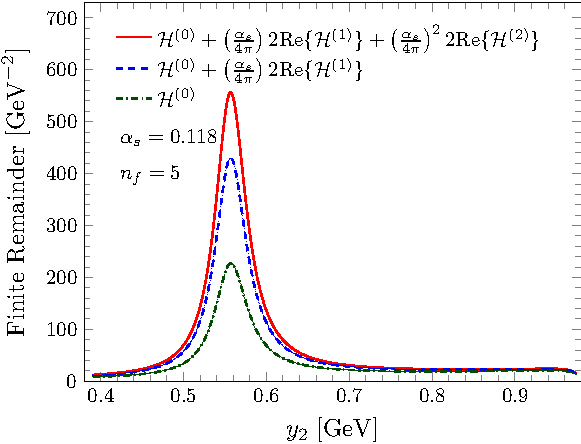
\includegraphics[width=.9\textwidth]{finite_remainder_gg.pdf}
    \label{fig:gg}
    \caption{$\mathbf{gg}$}
\end{subfigure}%
\begin{subfigure}{.5\textwidth}
    \centering
    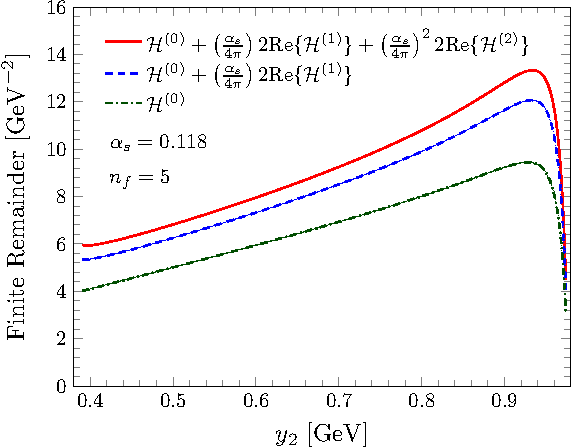
\includegraphics[width=.9\textwidth]{finite_remainder_qqx.pdf}
    \label{fig:qqx}
    \caption{$\mathbf{q\bar{q}}$}
\end{subfigure}
\begin{subfigure}{.5\textwidth}
    \centering
    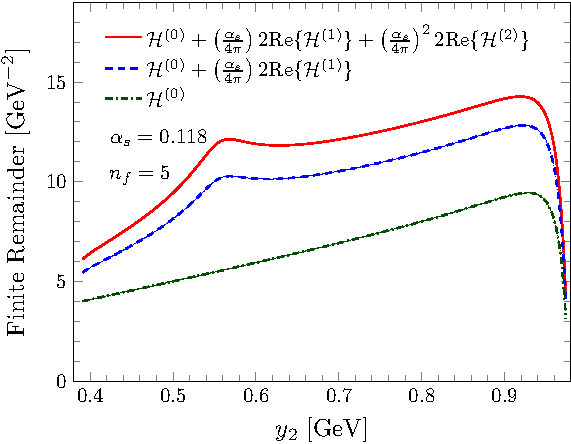
\includegraphics[width=.9\textwidth]{finite_remainder_qxq.pdf}
    \label{fig:qxq}
    \caption{$\mathbf{\bar{q}q}$}
\end{subfigure}%
\begin{subfigure}{.5\textwidth}
    \centering
    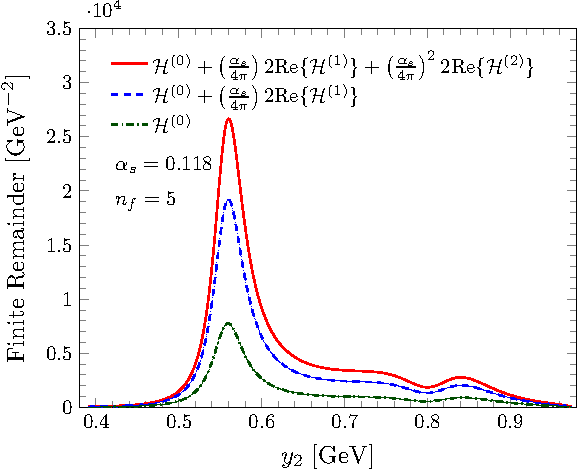
\includegraphics[width=.9\textwidth]{finite_remainder_bb.pdf}
    \label{fig:bb}
    \caption{$\mathbf{bb}$}
\end{subfigure}
\begin{subfigure}{.5\textwidth}
    \centering
    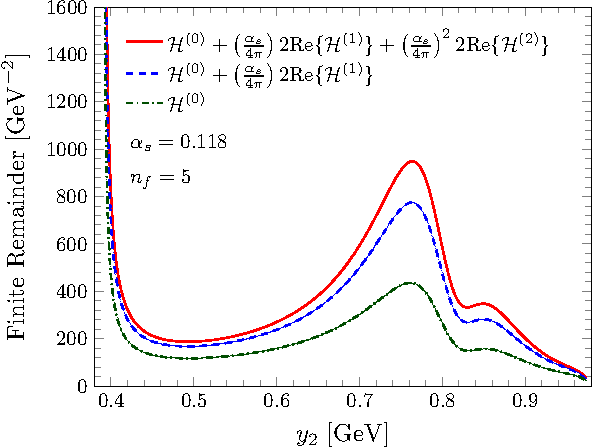
\includegraphics[width=.9\textwidth]{finite_remainder_bbx.pdf}
    \label{fig:bbx}
    \caption{$\mathbf{b\bar{b}}$}
\end{subfigure}%
\begin{subfigure}{.5\textwidth}
    \centering
    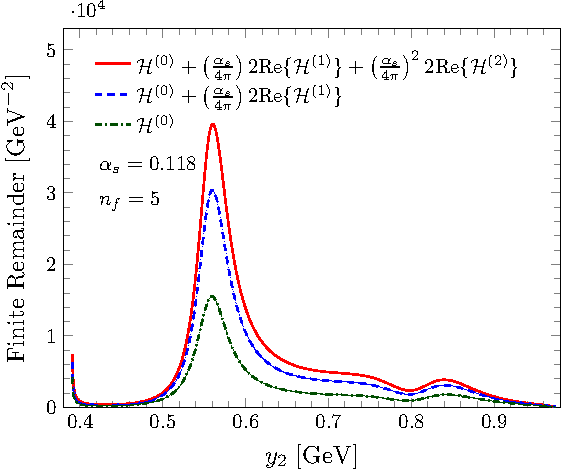
\includegraphics[width=.9\textwidth]{finite_remainder_bxb.pdf}
    \label{fig:bxb}
    \caption{$\mathbf{\bar{b}b}$}
\end{subfigure}
\caption[short]{Reduced squared finite remainders $\mathcal{H}^{(L)}$ at tree level, one and two loops evaluated on the one-dimensional phase space slice defined 
in Eq.~\ref{eq:parametrisation}, as functions of the variable $y_2$, for the channels defined in Eq.~\ref{eq:channel_definition}.}
\label{fig:plots}
\end{figure}

We stress that the purpose of the plots in Fig.~\ref{fig:plots} is merely to demonstrate that our results for the finite remainders can be evaluated reliably in the physical scattering region. Nothing can be inferred about the convergence of the perturbative expansion at the cross section level. One interesting feature which can be appreciated from Fig.~\ref{fig:plots} is the appearance of a loop-induced peak in the finite remainders for the channel $\mathbf{\bar{q}q}$. The peak is absent at tree level for the same channel and up to two loops for $\mathbf{q\bar{q}}$. The latter channel is related to $\mathbf{\bar{q}q}$ by the exchange $3\leftrightarrow 4$ of the external particles. We observe that the peak stems from the values of the finite remainder function basis, while the rational coefficients are not enhanced in that region. In order to pinpoint more precisely the origin of this phenomenon, we construct the explicit analytic expressions for some of the special functions which exhibit the peak, starting from their iterated integral expression obtained by solving the system of canonical DEs Eq.~\ref{eq:dh}. For instance:
\begin{align} \label{eq:h24}
h^{(2)}_4 & = 2 \, \text{Li}_2\left( 1 - \frac{s_{15}}{p_5^2} \right) + 2 \, \text{Li}_2 \left( 1- \frac{s_{23}}{s_{15}}\right) -\frac{\pi^2}{4} + \frac{1}{2} \log^2\left( p_5^2 \right) + \frac{1}{2}\log^2\left( -s_{45}\right) + 2 \log^2\left( s_{15}\right) \nonumber \\
& - \frac{1}{2}\log^2\left( -s_{23}\right) - 2 \log\left( s_{15}\right) \log\left( s_{15} - s_{23}\right) + \log^2\left( s_{15} - s_{23}\right) + \log\left( p_5^2\right) \log\left(-s_{23}\right) \nonumber \\
& - 2 \log\left( p_5^2\right) \log\left(s_{15} \right)  - \log\left( p_5^2\right) \log\left( -s_{14}\right) +2 \log\left( s_{15}\right) \log\left( -s_{14}\right) 
 - \log\left(-s_{23}\right) \log\left( -s_{14}\right) \nonumber \\
 & +i \pi \biggl[ \log\left( p_5^2\right) - 2 \log\left( s_{15}\right) + 2 \log\left( s_{15} - s_{23}\right) - \log\left( -s_{23}\right) - \log\left( -s_{14}\right)\biggr] \,,
\end{align}
which is well defined in the $s_{34}$ physical scattering region. The analytic continuation to any other region is obtained by adding a small positive imaginary part to each $s_{ij}$ and to $p_5^2$. We checked that the values of $h^{(2)}_4$ as given by Eq.~\ref{eq:h24} (and of its permutations) agree with the evaluation through the generalised series expansion. The function $h^{(2)}_4$ exhibits no peak on the phase space sliced defined by Eqs.~\ref{eq:parametrisation} and~\ref{eq:fixparameters}, and indeed the finite remainder for the channel $\mathbf{q\bar{q}}$ does not exhibit such feature. The permutation $3\leftrightarrow 4$ of $h^{(2)}_4$, which contributes to $\mathbf{\bar{q}q}$, is instead peaked around $y_2 \approx 0.5566$. Thanks to the analytic expression Eq.~\ref{eq:h24}, we can identify the source of the peak in the logarithms of $s_{24}$, which originate from the $\log (-s_{23})$'s in Eq.~\ref{eq:h24} upon swapping $3\leftrightarrow 4$. Indeed, the tree-level amplitude for the subprocess $0\to\bar{b} b \bar{q} q H$, given by Eq.~\ref{eq:A0bbqqh}, is manifestly free of $1/\langle 23 \rangle$ poles. The $0\to\bar{b} b \bar{q} q H$ diagrams with a $1/s_{23}$ pole would come with a loop and so end up scaling as $\log(-s_{23})$. While $\log(-s_{23})$ is not enhanced on the one-dimensional slice under consideration, its $3\leftrightarrow4$ permutation $\log(-s_{24})$, which contributes to $\mathcal{H}^{(L)}_{\mathbf{\bar{q}q}}$ for $L=1,2$, is peaked at $y_2 \approx 0.5566$, where $s_{24}$ reaches its minimum absolute value on the slice. 
The tree-level amplitudes for the channel $\mathbf{gg}$ instead do have poles at $s_{23}=0$, which
can be seen explicitly in Eqs.~\ref{eq:A0bbggh}. Since $\mathcal{H}^{(L)}_{\mathbf{gg}}$ with
$L=1,2$ receive contributions from the partial finite remainders in both the standard orientation
and with the swap $3\leftrightarrow4$, as shown in Eq.~\ref{eq:channel_gg}, their plot in Fig.~\ref{fig:plots}~(a) exhibits this peak already at tree level. The same holds for the $\mathbf{bb}$ and $\mathbf{\bar{b}b}$ channels, as can be seen in Figs.~\ref{fig:plots}~(d) and~(f). 

Also in Fig.~\ref{fig:plots}, we observe divergences at $y_2 = 39/100$ for the processes
$\mathbf{b\bar{b}}$ and $\mathbf{\bar{b}b}$. This divergence is associated with the propagator
$1/s_{12}$, which can only appear in processes with two pairs of bottom quarks. In Eqs.~\ref{eq:channel_bB}~and~\ref{eq:channel_Bb} 
we can see the $q\bar{q}$ fermion pairs can appear
with momenta $p_1$ and $p_2$, which is not the case for other processes. All the other features of the plots
in Fig.~\ref{fig:plots} can be similarly understood in terms of tree-level propagators going on shell.

\section{Summary}
\label{Hbbsec:conclusions}

In this chapter, we have presented an analytic form for the two-loop QCD corrections to the process
$pp\to b\bar{b}H$. To the best of our knowledge, this is the first complete set of helicity
amplitudes provided for a $2\to 3$ scattering process with an off-shell leg. A special function basis for
the finite remainder was identified obeying canonical form DEs. The method for
constructing such a basis was presented in the recent $pp\to Wb\bar{b}$ computation~\cite{Badger:2021nhg}. The finite remainders were then extracted from multiple
evaluations over finite fields and IBP reduction, with a rational parametrisation of the external kinematics.
We obtained relatively compact results after determining the linear relations between the rational coefficients and
performing a univariate partial fraction decomposition on the fly. The final expressions were evaluated using the method of generalised series expansions as implemented in the \texttt{DiffExp} code~\cite{Hidding:2020ytt}.

The expressions have been validated in a number of ways and we observe that they exhibit a smooth behaviour in all
scattering regions. Evaluation times appear to be suitable for phenomenological applications,
especially since we have not tried to optimise the route through the phase space evaluations as has
been done in other applications of the method~\cite{Frellesvig:2019byn,Abreu:2020jxa,Becchetti:2020wof,Bonciani:2021zzf,abreu2021twoloop}.

The techniques presented here show promise for applications to other important scattering processes such as $pp\to V+2j$ and $pp\to H+2j$. We point out that the bases of pure MIs required for the non-planar topologies needed in these computations have been recently made available in literature after the completion of our work~\cite{Abreu:2023rco}.

\end{document}